\documentclass[11pt]{article}

\usepackage[a4paper,margin=0.82in]{geometry}
\usepackage{amsmath,amssymb}
\usepackage{array}
\usepackage{booktabs}
\usepackage{caption}
\usepackage{enumitem}
\usepackage{fancyhdr}
\usepackage{float}
\usepackage{graphicx}
\usepackage[hidelinks]{hyperref}
\usepackage{listings}
\usepackage{longtable}
\usepackage{microtype}
\usepackage{siunitx}
\usepackage{xcolor}

\sisetup{
  group-separator={,},
  group-minimum-digits=4,
  detect-weight=true,
  detect-family=true
}

\definecolor{darkblue}{RGB}{21,57,92}
\definecolor{darkgray}{RGB}{53,64,75}
\definecolor{codebg}{RGB}{248,249,251}
\definecolor{codeframe}{RGB}{203,210,217}

\lstdefinestyle{pythoncode}{
  language=Python,
  basicstyle=\ttfamily\scriptsize,
  backgroundcolor=\color{codebg},
  frame=single,
  rulecolor=\color{codeframe},
  numbers=left,
  numberstyle=\tiny\color{darkgray},
  numbersep=6pt,
  xleftmargin=1.2em,
  framexleftmargin=1em,
  breaklines=true,
  breakatwhitespace=false,
  columns=fullflexible,
  keepspaces=true,
  showstringspaces=false,
  tabsize=4,
  captionpos=b
}

\pagestyle{fancy}
\fancyhf{}
\lhead{\textcolor{darkgray}{IEDA4331 Crypto Options Project}}
\rhead{\textcolor{darkgray}{Crypto Option Model Comparison}}
\cfoot{\thepage}

\setlength{\parindent}{0pt}
\setlength{\parskip}{6pt}
\setlist[itemize]{leftmargin=1.15em,itemsep=2pt,topsep=2pt}

\title{\vspace{-1.0cm}\textbf{\textcolor{darkblue}{Pricing, Greeks, and Jump-Risk Management for BTC/ETH Vanilla Options}}\\
\large IEDA4331 Financial Engineering Group Project}
\author{
Choi Man Hou\\
\texttt{mhchoiaf@connect.ust.hk}\\
SID: 20894196
\and
Lee Cheuk Yiu\\
\texttt{cyleebt@connect.ust.hk}\\
SID: 21051040
}
\date{Market data snapshot: 2026-05-19 19:26 UTC}

\begin{document}
\maketitle

\begin{abstract}
This report prices BTC and ETH vanilla options using the core IEDA4331 toolkit: risk-neutral valuation, Black-Scholes pricing, CRR binomial trees, implied volatility, Greeks, and dynamic hedging. We treat the Merton jump-diffusion model as a classical jump benchmark rather than the final innovation. The modern exploration layer then evaluates four crypto-relevant candidates at the same empirical level: stochastic volatility with correlated jumps, market-regime implied stochastic volatility, time-varying jump intensity, and GARCH option pricing. The calibrated Merton benchmark reduces mean absolute pricing error by 80.0\% for BTC and 58.2\% for ETH relative to a historical-volatility Black-Scholes baseline. The refreshed equal-level comparison is deliberately nuanced: \textbf{Merton gives the lowest BTC MAE}, \textbf{MR-ISVM gives the lowest ETH MAE}, \textbf{SVCJ produces the largest standardized crash-protection premium}, and hedge-error leadership depends on the asset and risk objective. The main conclusion is that crypto option markets price non-Gaussian jump and volatility-regime risk explicitly; Black-Scholes remains a necessary no-arbitrage benchmark, but it is not sufficient as a standalone crypto risk engine.
\end{abstract}

\newpage
\tableofcontents
\newpage

\section{Introduction and Course Motivation}

This report studies BTC and ETH vanilla options under the central language of IEDA4331: no-arbitrage pricing, risk-neutral valuation, binomial replication, the Black-Scholes-Merton PDE, implied volatility, Greeks, and hedging error. The objective is to move from classroom pricing identities to a market-calibrated crypto option risk engine, then ask where the classical diffusion model fails. We use the Black-Scholes model \cite{blackscholes1973,merton1973}, CRR binomial tree \cite{coxrossrubinstein1979}, and Merton jump-diffusion model \cite{merton1976} as the classical ladder of benchmarks.

The Risk-Neutral Pricing chapter brings the analysis from physical expected returns to martingale valuation. Instead of asking whether BTC or ETH is expected to appreciate, we price contingent claims under $Q$:
\[
V_t=E_t^Q\!\left[e^{-r(T-t)}V_T\right].
\]
The Binomial Tree chapter brings the analysis to finite-state replication: a derivative is priced by constructing a self-financing portfolio whose future payoff matches the claim. The Black-Scholes-Merton chapter then takes the limiting continuous-time view and derives the PDE from a self-financing delta hedge:
\[
\frac{\partial V}{\partial t}
+rS\frac{\partial V}{\partial S}
+\frac{1}{2}\sigma^2S^2\frac{\partial^2V}{\partial S^2}
-rV=0.
\]
The Risk Management chapter brings the analysis from valuation to control: Delta, Gamma, Vega, discrete hedging error, VaR logic, and stress testing. Our report follows that course arc, then adds a jump process precisely where the diffusion assumption breaks down for cryptocurrency markets.

\section{Data and Market Snapshot}

We use public Deribit data for BTC and ETH:
\texttt{get\_book\_summary\_by\_currency} for option books,
\texttt{get\_instruments} for contract metadata, and
\texttt{get\_index\_chart\_data} for one-year index histories. Deribit option premiums are quoted in coin units, so we convert them into USD:
\[
\text{Option price}_{USD}=\text{Option price}_{coin}\times S.
\]

\begin{table}[H]
\centering
\caption{Deribit option universe after cleaning}
\begin{tabular}{lrrrrrr}
\toprule
Currency & Raw rows & Usable rows & Median spot & Median IV & Min days & Max days\\
\midrule
BTC & 878 & 688 & 76975.3 & 42.13\% & 1.52 & 310.5\\
ETH & 710 & 474 & 2118.6 & 55.29\% & 1.52 & 310.5\\
\bottomrule
\end{tabular}
\end{table}

\begin{figure}[H]
\centering
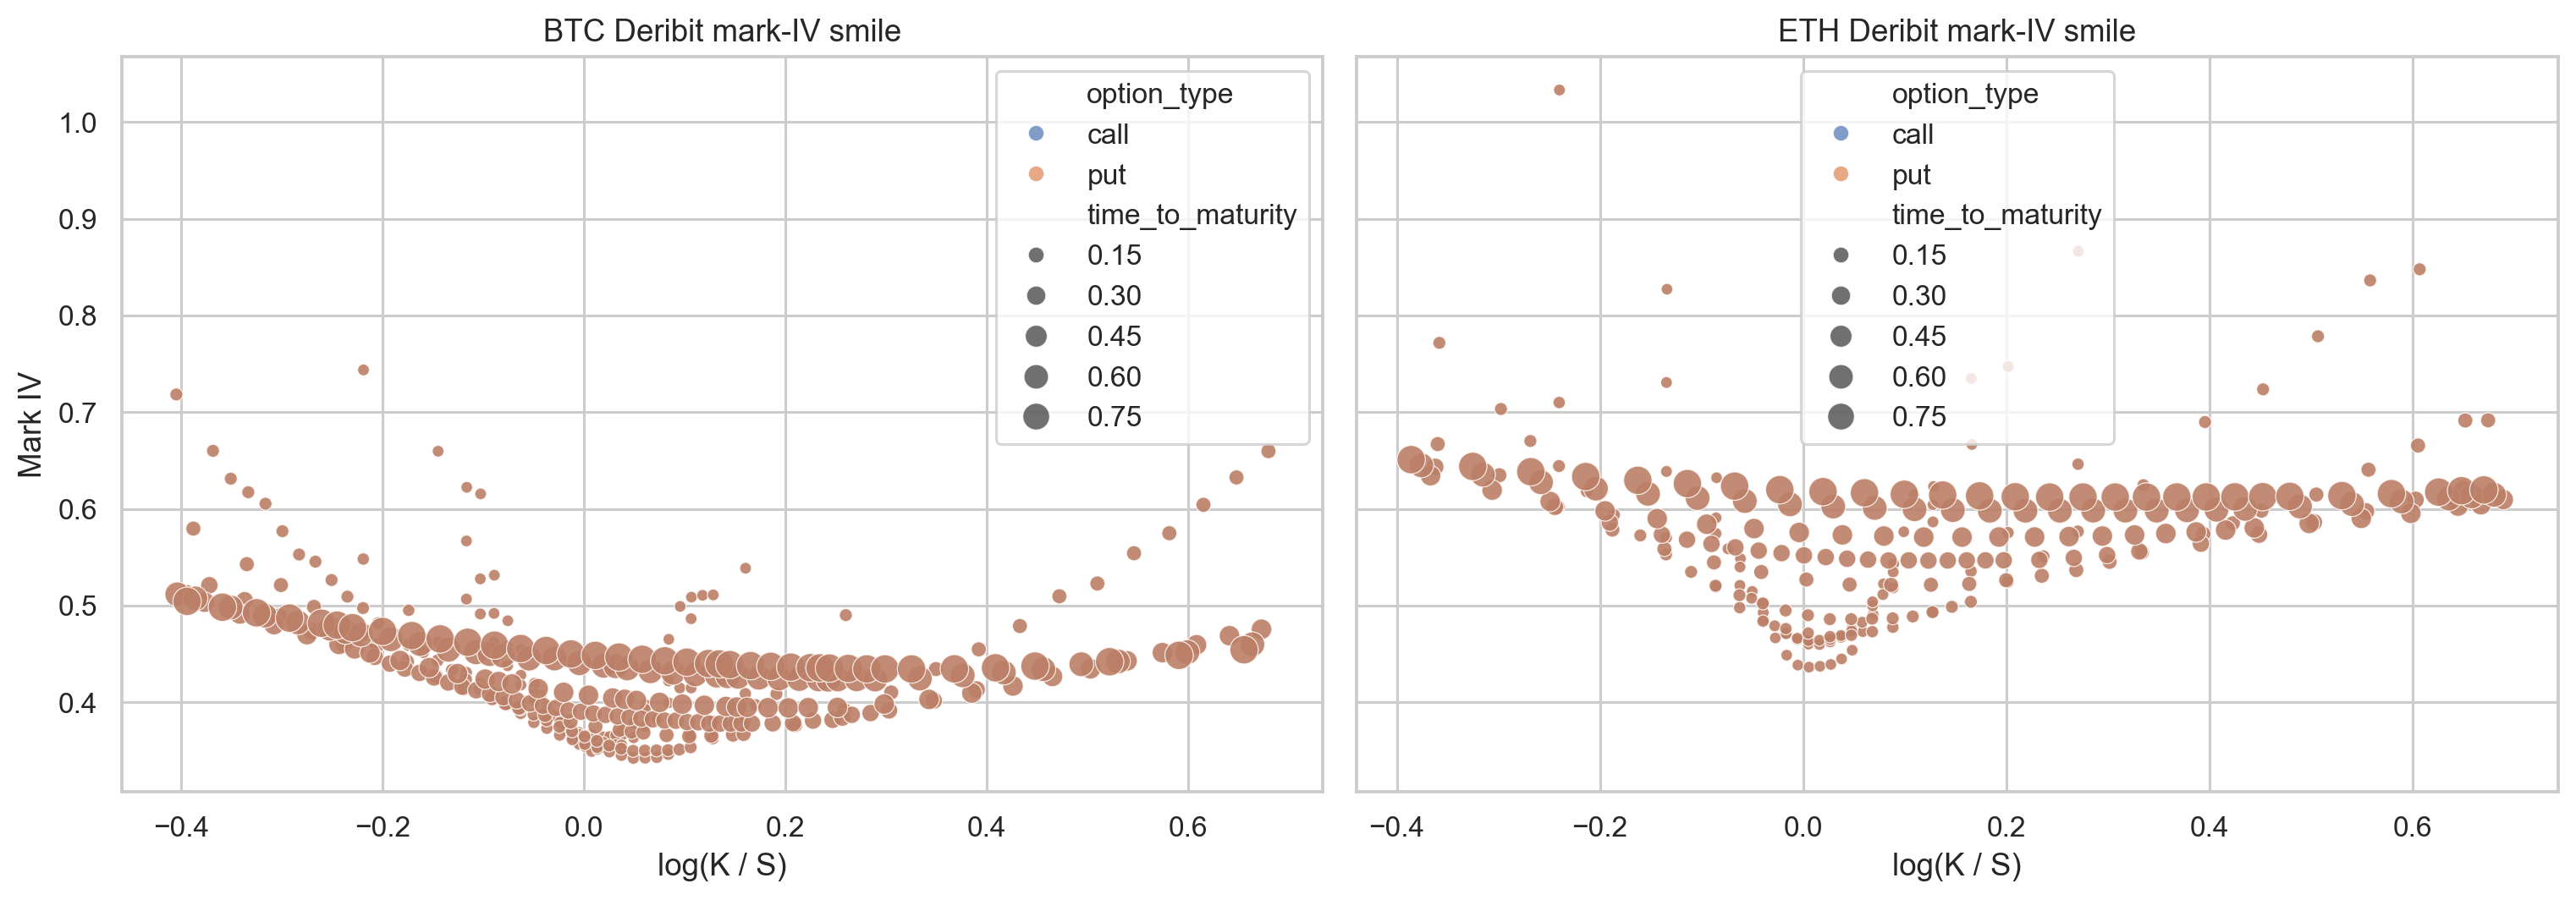
\includegraphics[width=0.98\linewidth]{figures/02_deribit_iv_smiles.png}
\caption{Deribit mark implied-volatility smiles across strikes and maturities.}
\end{figure}

\textbf{Inference.} A flat Black-Scholes volatility input would imply a roughly horizontal surface. The observed BTC and ETH smiles are curved and dispersed, indicating that the market prices skew, maturity effects, and non-Gaussian tail risk.

The course's implied-volatility concept is important here. Implied volatility is not simply another volatility estimator; it is the volatility that forces the Black-Scholes formula to match a traded option price. A smile therefore means the market is using Black-Scholes as a quote convention while rejecting its constant-volatility distributional assumption. Crypto option studies document precisely this pattern in Bitcoin options \cite{zulfiqar2021iv,chenyang2024}. This is the bridge from the data section to the model-innovation section.

\textbf{Comparative lens.} The same smile carries different information for each model. Black-Scholes treats it as model error; Merton and dynamic jump intensity read it as evidence of discontinuous tail risk; MR-ISVM reads it as a state-dependent surface; GARCH reads it as volatility clustering; and SVCJ reads it as joint spot-volatility stress.

\section{Evaluation Metrics and Comparative Protocol}

To keep the candidate comparison at the same level throughout the report, every model is evaluated on the same cleaned option universe. For option $i$, let $V_i^{mkt}$ denote the Deribit USD market price and $\widehat{V}_{i}^{(m)}$ denote the price produced by model $m$. The model pricing error is:
\[
e_i^{(m)}=\widehat{V}_{i}^{(m)}-V_i^{mkt}.
\]

The key cross-sectional pricing metrics are:
\[
\mathrm{Bias}^{(m)}=\frac{1}{N}\sum_{i=1}^{N}e_i^{(m)},
\]
\[
\mathrm{MSE}^{(m)}=\frac{1}{N}\sum_{i=1}^{N}\left(e_i^{(m)}\right)^2,
\qquad
\mathrm{RMSE}^{(m)}=\sqrt{\mathrm{MSE}^{(m)}},
\]
\[
\mathrm{MAE}^{(m)}=\frac{1}{N}\sum_{i=1}^{N}\left|e_i^{(m)}\right|,
\qquad
\mathrm{MedAE}^{(m)}=\mathrm{median}_{i}\left(\left|e_i^{(m)}\right|\right),
\]
\[
\mathrm{P90AE}^{(m)}=Q_{0.90}\left(\left|e_i^{(m)}\right|\right).
\]
MAE is the main headline metric because it is in USD units and is less dominated by a small number of very expensive contracts than MSE. RMSE is still reported because it penalizes large pricing misses more aggressively.

For pairwise improvement against Black-Scholes, we use:
\[
\Delta \mathrm{AE}_i^{(m)}
=
\left|e_i^{BS}\right|-\left|e_i^{(m)}\right|,
\qquad
\mathrm{ShareImproved}^{(m)}
=
\frac{1}{N}\sum_{i=1}^{N}\mathbf{1}\{\Delta \mathrm{AE}_i^{(m)}>0\}.
\]
The paired tests in the calibration section test whether $\Delta \mathrm{AE}_i^{(m)}$ is significantly positive for each candidate model.

For standardized crash protection, we price a 30-day 5\% out-of-the-money put under each model and define its model premium over Black-Scholes as:
\[
\mathrm{CrashPremium}^{(m)}
=
\widehat{V}^{(m)}_{\text{30d, 5\% OTM put}}
-
\widehat{V}^{BS}_{\text{30d, 5\% OTM put}}.
\]

For hedge simulations, each path $p$ produces a final short-option hedge P\&L, denoted $\mathrm{PnL}_p^{(m)}$. We summarize hedging with:
\[
\mathrm{MeanAbsHedgeError}^{(m)}
=
\frac{1}{P}\sum_{p=1}^{P}\left|\mathrm{PnL}_p^{(m)}\right|,
\qquad
\mathrm{LeftTail}_{5\%}^{(m)}
=
Q_{0.05}\left(\mathrm{PnL}_p^{(m)}\right).
\]
The first metric measures average replication error; the second measures adverse tail loss.

\section{Baseline Pricing Framework}

\subsection{Black-Scholes Benchmark}

For European calls and puts with no dividend yield:
\[
C=SN(d_1)-Ke^{-rT}N(d_2),\qquad
P=Ke^{-rT}N(-d_2)-SN(-d_1),
\]
where
\[
d_1=\frac{\log(S/K)+(r+\sigma^2/2)T}{\sigma\sqrt{T}},
\qquad
d_2=d_1-\sigma\sqrt{T}.
\]
Volatility is estimated from log returns, following the course treatment that log returns aggregate naturally across time and that annualized volatility scales with the square root of time. The physical drift is not used directly in risk-neutral pricing because the Black-Scholes PDE and risk-neutral valuation remove $\mu$ through replication.

\subsection{CRR Binomial Tree}

The CRR tree uses
\[
u=e^{\sigma\sqrt{\Delta t}},\qquad
d=\frac{1}{u},\qquad
p_Q=\frac{e^{r\Delta t}-d}{u-d}.
\]
At each node:
\[
V_t=e^{-r\Delta t}\bigl(p_QV_u+(1-p_Q)V_d\bigr).
\]
For American options, the backward step replaces continuation value with
\[
V_t=\max\{\text{continuation value},\text{ immediate exercise value}\}.
\]

This matters because the binomial tree is not only a numerical method. It is the discrete version of the course's no-arbitrage argument: $p_Q$ is not the real-world probability that BTC or ETH goes up, but the probability that makes discounted prices consistent with replication.

\begin{figure}[H]
\centering
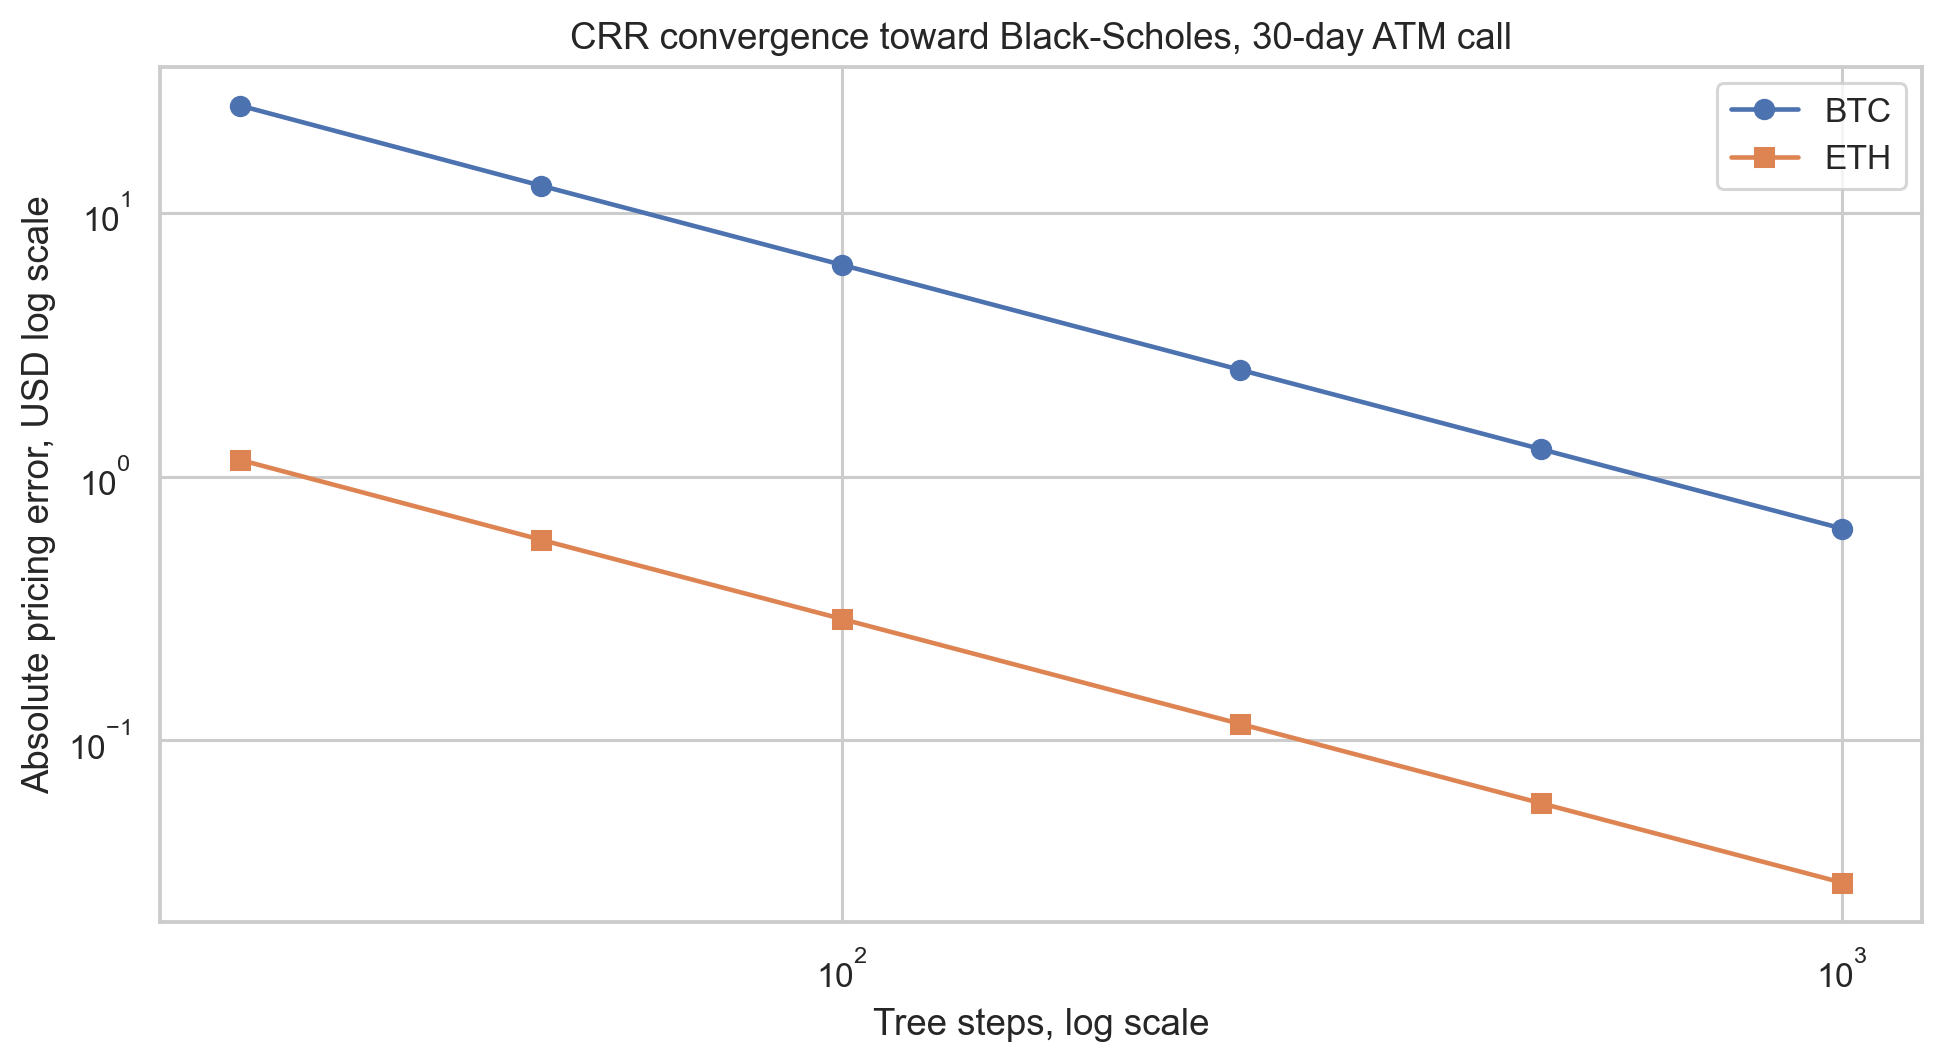
\includegraphics[width=0.82\linewidth]{figures/04_btm_convergence.png}
\caption{CRR convergence toward the Black-Scholes benchmark for 30-day at-the-money calls.}
\end{figure}

\begin{table}[H]
\centering
\caption{European and American CRR pricing, 30-day at-the-money options}
\begin{tabular}{llrrrrr}
\toprule
Currency & Option & Spot/Strike & BS Eur. & CRR Eur. & CRR Am. & Am. premium\\
\midrule
BTC & call & 76975.3 & 2449.75 & 2448.54 & 2448.54 & 0.00\\
BTC & put  & 76975.3 & 2386.55 & 2385.34 & 2388.59 & 3.25\\
ETH & call & 2118.6  & 107.37  & 107.32  & 107.32  & 0.00\\
ETH & put  & 2118.6  & 105.64  & 105.58  & 105.67  & 0.09\\
\bottomrule
\end{tabular}
\end{table}

\textbf{Inference.} The American call premium is effectively zero for non-dividend underlyings, while American puts carry a small early-exercise premium. This is exactly the qualitative result expected from the course theory: early exercise destroys call time value when there is no dividend benefit, but it can be rational for puts when the option is sufficiently in the money.

\textbf{Comparative role.} Black-Scholes and CRR are deliberately kept as the control models. They are not expected to win the crypto smile contest; their role is to anchor no-arbitrage logic, expose how far a diffusion benchmark misses market prices, and make later candidate improvements economically interpretable.

\section{Candidate Model Formulations}

\subsection{Merton as Classical Jump Benchmark}

The Merton jump-diffusion model was introduced in 1976 \cite{merton1976}. It is therefore not recent enough to be the final innovation by itself. In this report, it serves as the first serious extension beyond Black-Scholes: a classical benchmark that tests whether explicit price jumps improve crypto option pricing.

The model replaces the diffusion-only assumption with:
\[
\frac{dS_t}{S_{t^-}}=(r-\lambda\kappa)dt+\sigma dW_t^Q+(J-1)dN_t,
\]
where
\[
\log J\sim N(\mu_J,\delta_J^2),\qquad
\kappa=E[J-1]=e^{\mu_J+\frac{1}{2}\delta_J^2}-1.
\]
Here $\lambda$ is the annual jump intensity, $\mu_J$ is average log jump size, and $\delta_J$ is jump-size volatility. The compensator $\lambda\kappa$ keeps the discounted stock price consistent with risk-neutral valuation.

Conditional on $n$ jumps, terminal log-price remains Gaussian. Hence the Merton option value is a Poisson mixture of conditional Black-Scholes-style prices:
\[
V^{Merton}(S,K,T)=
\sum_{n=0}^{\infty}
e^{-\lambda T}\frac{(\lambda T)^n}{n!}V^{BS}_n(S,K,T).
\]
This extension preserves the course's risk-neutral framework while adding a realistic channel for crypto discontinuities. The compensator is essential: without it, the jump term would change the drift of the discounted stock process and break the martingale logic that motivates risk-neutral pricing.

\subsection{Candidate A: Stochastic Volatility with Correlated Jumps}

The first modern candidate is a stochastic volatility with correlated jumps (SVCJ) model. This model family is closely related to affine jump-diffusion work in option pricing \cite{bates1996,duffie2000}, and it has been applied directly to cryptocurrency options in recent empirical work \cite{hou2020crypto}. Its core idea is that crypto crashes are not only spot-price jumps; they are often volatility events as well.

A compact SVCJ specification is:
\[
\frac{dS_t}{S_{t^-}}
=(r-\lambda \mu_S)dt+\sqrt{v_t}\,dW_t^S+Y_t^S dN_t,
\]
\[
dv_t=\kappa_v(\theta_v-v_t)dt+\xi\sqrt{v_t}\,dW_t^v+Y_t^v dN_t,
\qquad
dW_t^S dW_t^v=\rho\,dt.
\]
Here $v_t$ is stochastic variance, $\rho$ captures leverage/skew, and $(Y_t^S,Y_t^v)$ allows price jumps and volatility jumps to arrive together. Compared with Merton, SVCJ can explain a more realistic crypto stress state:
\[
\text{spot falls sharply}\quad+\quad\text{implied volatility jumps upward}.
\]
In the implemented proxy, the historical return series initializes $v_0$, $\theta_v$, $\kappa_v$, variance-jump size, and leverage correlation. The option calibration then refines only the parameters that enter the moment-matched pricing equation directly: the variance multiplier and vol-of-vol $\xi$. This avoids an unidentified calibration problem: $\rho$ is economically important for skew, but in our reduced moment proxy it is reported as a historical state estimate rather than optimized as if it affected prices.

\subsection{Candidate B: Market-Regime Implied Stochastic Volatility}

The second candidate is a market-regime implied stochastic volatility model (MR-ISVM), motivated by recent crypto option research \cite{saef2022mrisvm}. The key idea is that crypto option surfaces behave differently across regimes such as calm markets, trending markets, and stress markets. A reduced formulation is:
\[
z_t\in\{1,\ldots,M\},\qquad
\sigma_{\mathrm{IV}}(K,T,t)=f_{z_t}(K,T),
\]
\[
V_t=BS\!\left(S_t,K,T,r,\sigma_{\mathrm{IV}}(K,T,t)\right).
\]
The regime variable $z_t$ can be estimated from returns, realized volatility, volume, or option-surface features. Compared with Merton, MR-ISVM does not force one set of jump parameters to explain all market states; it allows the implied volatility surface itself to become state-dependent.

Our fitted MR-ISVM surface uses a 12-factor design in log-moneyness $x=\log(K/S)$:
\[
\begin{aligned}
\sigma_{\mathrm{IV}}
=\mathrm{clip}\big(&
\beta_0+\beta_1x+\beta_2|x|+\beta_3x^2+\beta_4\sqrt{T}+\beta_5T\\
&+\beta_6I_{put}+\beta_7I_{put}x+\beta_8I_{short}\\
&+\beta_9x\sqrt{T}+\beta_{10}I_{put}\sqrt{T}+\beta_{11}x^3,\,
\sigma_{\min}(T),\sigma_{\max}\big).
\end{aligned}
\]
The cross term $x\sqrt{T}$ lets skew vary by maturity, $I_{put}\sqrt{T}$ lets the put wing have a different term slope, and $x^3$ adds asymmetric wing curvature. This specification makes MR-ISVM more than a static smile fit: it becomes a regime-aware and maturity-aware surface benchmark that can be compared directly with structural jump and volatility models.

\subsection{Candidate C: Time-Varying Jump Intensity}

The third candidate is a dynamic jump-intensity model. Recent Bitcoin option evidence emphasizes that jump magnitude and jump arrival rates are time-varying \cite{chenyang2024}. This is important for crypto because large moves can cluster through leverage, liquidations, and margin pressure.

A parsimonious extension is:
\[
\frac{dS_t}{S_{t^-}}=(r-\lambda_t\kappa)dt+\sigma dW_t^Q+(J-1)dN_t,
\]
\[
d\lambda_t=\beta(\bar{\lambda}-\lambda_t)dt+\alpha\,dN_t.
\]
After a jump, $\lambda_t$ increases, then mean-reverts. Compared with Merton's constant $\lambda$, this model captures jump clustering and liquidation-cascade risk.

\subsection{Candidate D: GARCH Option Pricing}

The fourth candidate is a GARCH option-pricing model, which has also been studied for Bitcoin options \cite{venter2020garch}. It is a discrete-time alternative that connects naturally to the course's historical volatility estimation section:
\[
r_{t+1}=\mu+\sqrt{h_{t+1}}\varepsilon_{t+1},
\]
\[
h_{t+1}=\omega+\alpha r_t^2+\beta h_t.
\]
Option prices can then be computed by simulation under a risk-neutralized conditional variance process. Compared with Merton, GARCH does not require discontinuous jumps, but it captures volatility clustering. It is therefore useful as a competing explanation for smiles: are crypto smiles mainly jump risk, or time-varying volatility?

\begin{table}[H]
\centering
\caption{Equal-level implementation protocol for all candidate models}
\small
\begin{tabular}{p{0.15\linewidth}p{0.23\linewidth}p{0.27\linewidth}p{0.25\linewidth}}
\toprule
Model & Calibration object & Pricing engine & Same-level diagnostic\\
\midrule
Black-Scholes & Historical log-return variance & Closed-form diffusion formula & Full-universe MAE/RMSE and Greeks\\
Merton & Weighted Deribit option-price error & Poisson mixture of Black-Scholes prices & Full-universe MAE/RMSE, jump sensitivity, hedging\\
SVCJ proxy & Historical variance state plus identifiable variance and $\xi$ calibration & Moment-matched stochastic variance with Merton jumps & Full-universe MAE/RMSE and standardized crash put\\
MR-ISVM & Regime-aware Deribit mark-IV cross section & Black-Scholes with active-regime fitted IV surface & Full-universe MAE/RMSE and standardized crash put\\
Dynamic jump & Weighted option-price error with mean-reverting $\lambda_t$ & Merton mixture with horizon-dependent effective intensity & Full-universe MAE/RMSE and standardized crash put\\
GARCH & Historical conditional return variance & Black-Scholes with forecast average variance & Full-universe MAE/RMSE and standardized crash put\\
\bottomrule
\end{tabular}
\end{table}

This protocol is deliberately symmetric. Each candidate uses the same cleaned Deribit universe, the same 80-contract calibration discipline where option calibration is needed, and the same diagnostic definitions from the previous section. The SVCJ implementation is labelled as a proxy because a full affine SVCJ calibration normally requires a time series of option surfaces; here we use a moment-matched variance state so it can be compared fairly with the available live snapshot. The empirical comparison is then carried through the distribution, calibration, sensitivity, Greeks, and hedging sections rather than isolated here.

\begin{table}[H]
\centering
\caption{Regime-aware MR-ISVM surface diagnostics}
\small
\begin{tabular}{llrrrr}
\toprule
Currency & Active regime & Calibrated regimes & Coefficients & Rel. price RMSE & IV floor/cap\\
\midrule
BTC & stress & calm, trend & 12 & 0.3699 & 0.20 / 3.00\\
ETH & stress & calm, stress & 12 & 0.2783 & 0.20 / 3.00\\
\bottomrule
\end{tabular}
\end{table}

\textbf{Model-design inference.} Both assets are detected in stress regimes in this snapshot. ETH has a directly fitted stress surface, while BTC falls back to fitted calm/trend surfaces because the stress slice is sparse in the live option snapshot. This is exactly why the surface model is useful in a course project: the Black-Scholes formula remains the pricing map, while the implied volatility input becomes a market-state object rather than a single scalar.

\section{Historical Distribution and Jump Diagnostics}

We compute one-year BTC/ETH log returns from Deribit index history. Jumps are detected using a robust z-score threshold of 4.0. Non-jump observations initialize diffusive volatility; jump observations initialize jump intensity and jump-size distribution.

\begin{figure}[H]
\centering
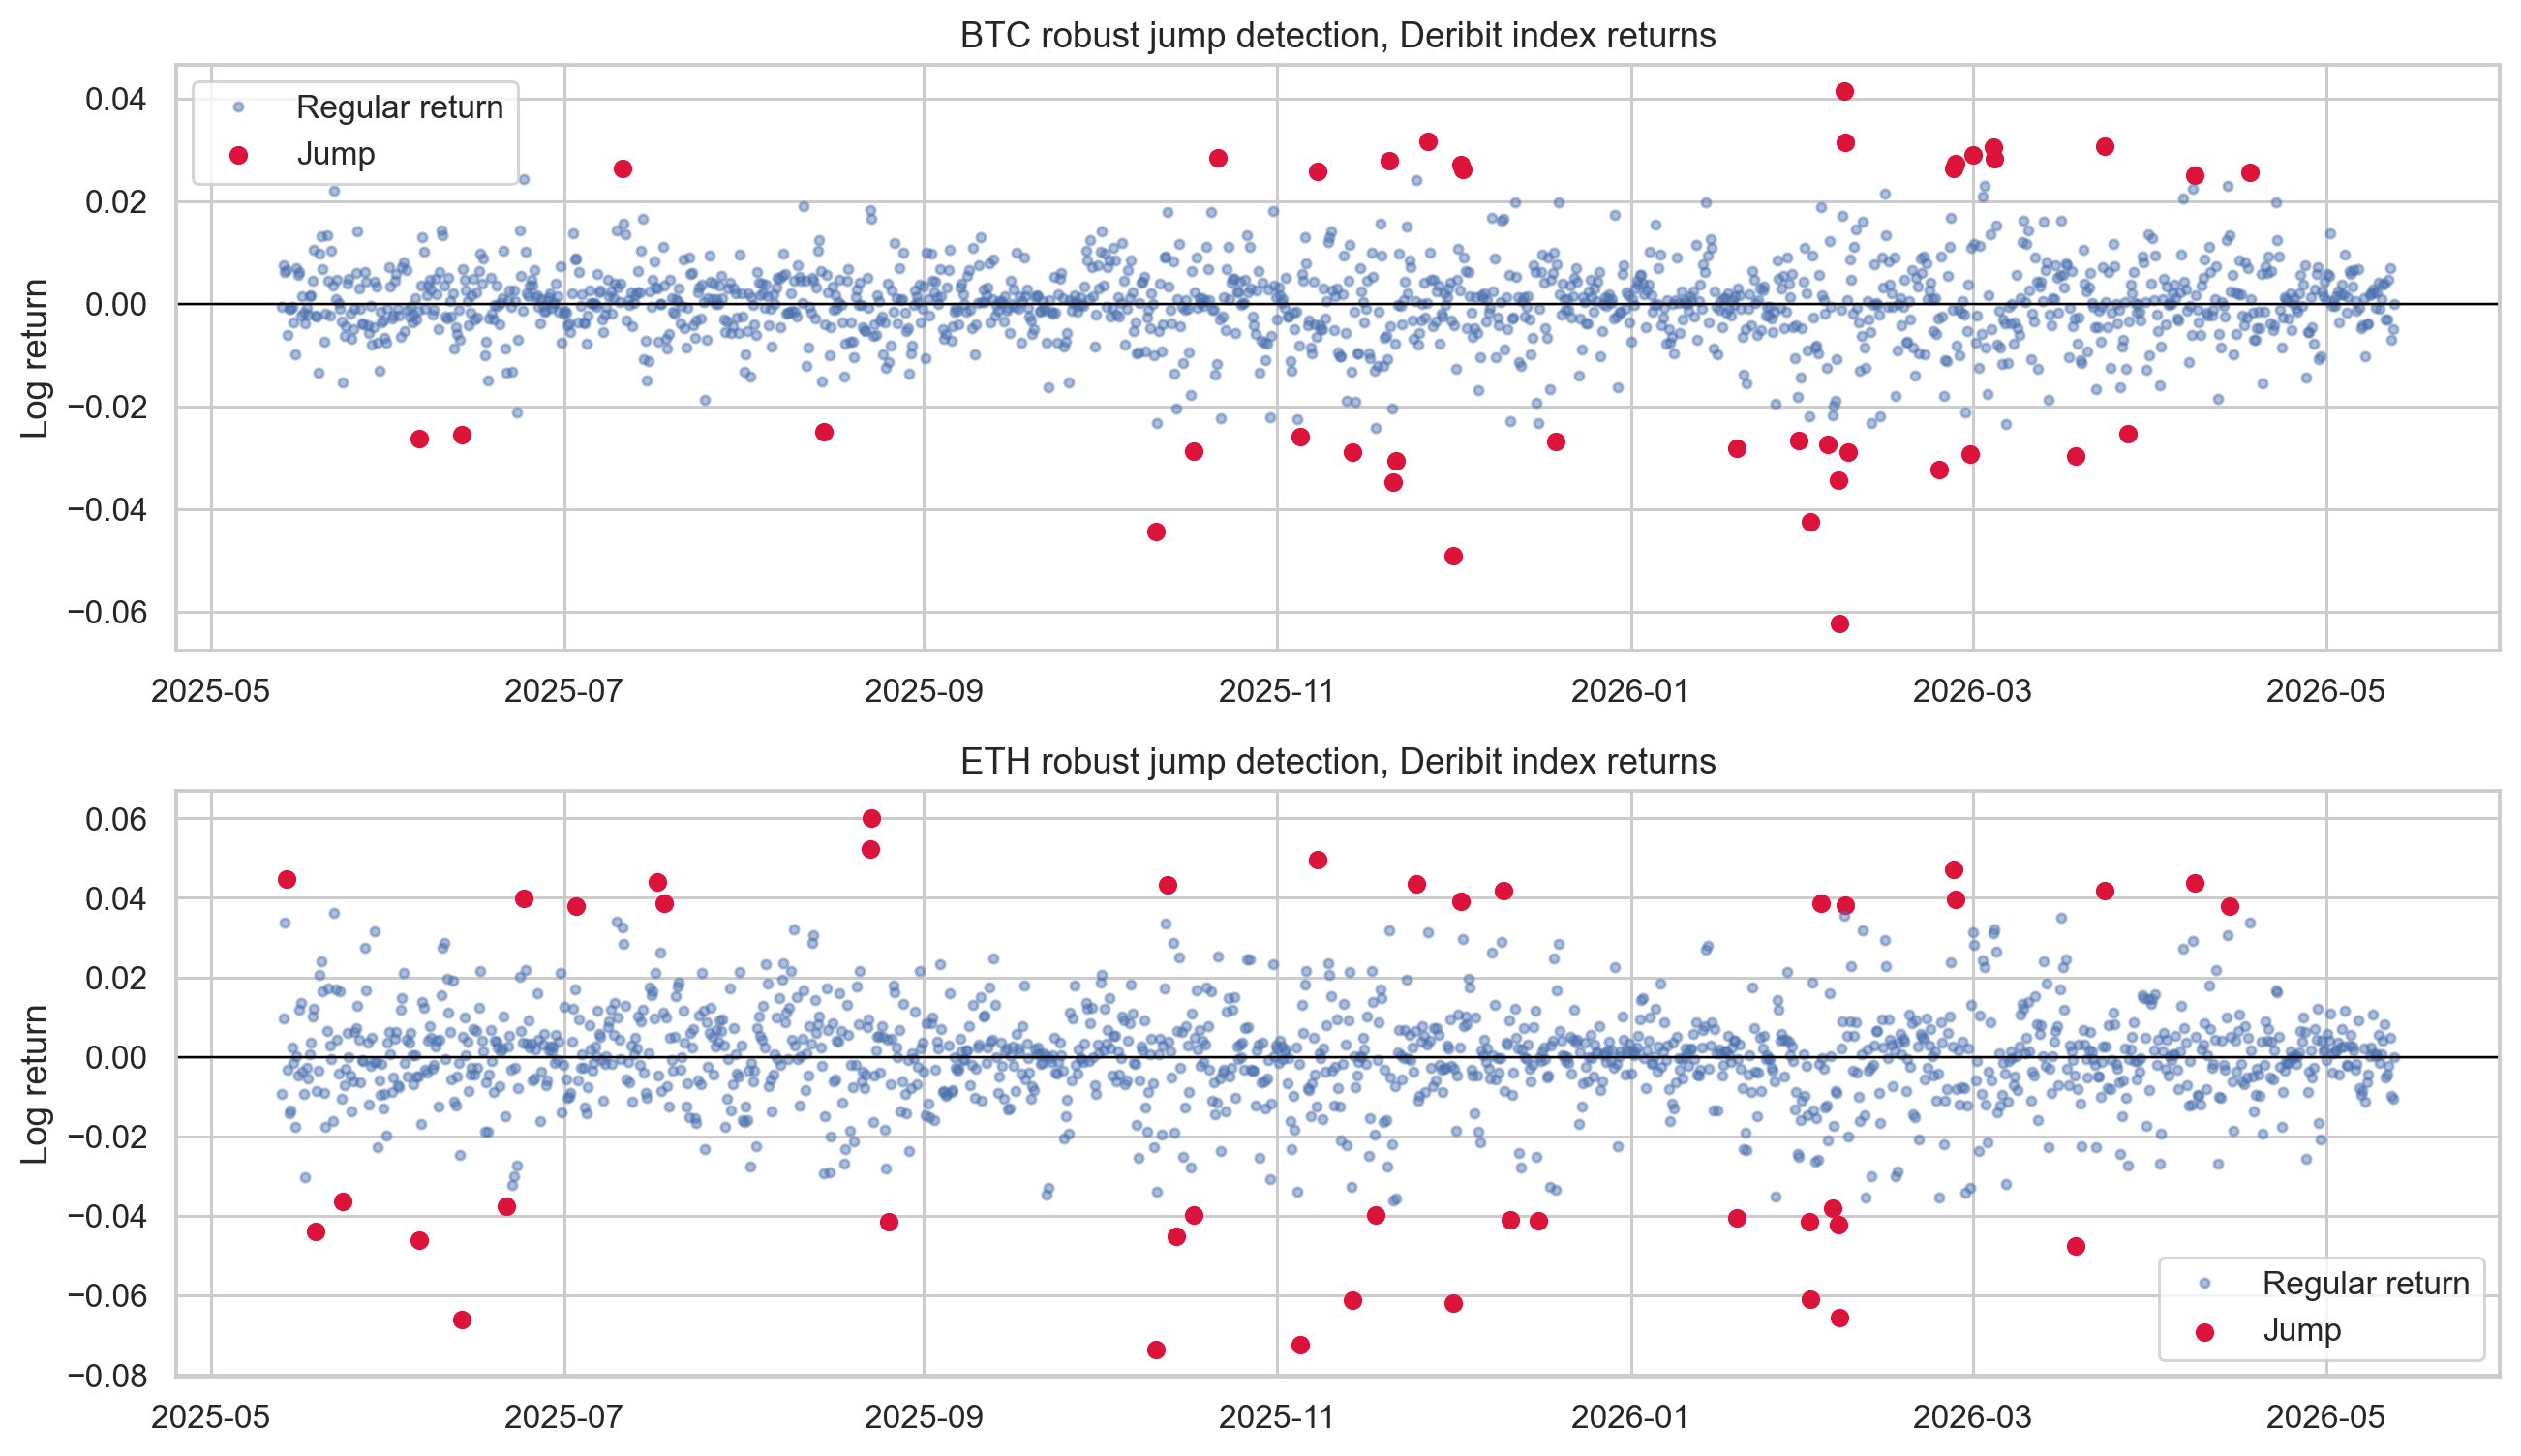
\includegraphics[width=0.98\linewidth]{figures/01_return_jump_detection.png}
\caption{Robust jump detection in BTC and ETH index log returns.}
\end{figure}

\begin{table}[H]
\centering
\caption{Historical jump initialization}
\begin{tabular}{lrrrrrrrr}
\toprule
Currency & Obs. & Jumps & Diff. $\sigma$ & $\lambda$ & $\mu_J$ & $\delta_J$ & Worst & Best\\
\midrule
BTC & 1459 & 40 & 27.49\% & 40.05 & -0.500\% & 3.157\% & -6.240\% & 4.139\%\\
ETH & 1459 & 40 & 44.02\% & 40.05 & -0.748\% & 4.746\% & -7.373\% & 6.014\%\\
\bottomrule
\end{tabular}
\end{table}

\begin{table}[H]
\centering
\caption{Return distribution diagnostics}
\begin{tabular}{lrrrrrr}
\toprule
Currency & Ann. mean & Ann. vol & Skew & Ex. kurtosis & JB statistic & JB p-value\\
\midrule
BTC & -32.55\% & 33.68\% & -0.547 & 4.918 & 1530.39 & $<10^{-12}$\\
ETH & -18.98\% & 52.79\% & -0.399 & 3.623 & 829.07 & $<10^{-12}$\\
\bottomrule
\end{tabular}
\end{table}

\textbf{Inference.} Jarque-Bera tests strongly reject normality for both BTC and ETH returns. Both assets exhibit negative skew and excess kurtosis, validating the modeling decision to go beyond a lognormal diffusion. ETH has higher annualized volatility and jump-size volatility, while BTC still exhibits material discontinuous downside risk.

This section deepens the Black-Scholes estimation chapter. In the classical model, the statistic we need is the standard deviation of log returns. For BTC/ETH, that statistic is still useful, but it is incomplete: skewness, kurtosis, and jump frequency explain why a single $\sigma$ cannot reproduce the market smile. The empirical distribution therefore motivates a pricing model with both a continuous volatility channel and a discontinuous jump channel.

\textbf{Comparative lens.} These diagnostics initialize different model states. Black-Scholes uses only diffusive volatility; Merton uses diffusive volatility plus jump intensity and jump-size moments; dynamic jump intensity asks whether $\lambda_t$ should vary across horizons; GARCH uses conditional variance persistence; SVCJ uses both variance state and variance-jump state; and MR-ISVM uses the option surface itself to infer the current regime.

\section{Market Calibration and Statistical Evidence}

Merton parameters are calibrated to liquid Deribit option marks by minimizing weighted relative pricing error. The calibration uses 80 liquid options per asset; diagnostics are computed on the full cleaned universe. Conceptually, this is an implied-parameter exercise: just as the course defines implied volatility by inverting Black-Scholes, we infer jump and volatility states by matching a cross-section of market option prices. The same cleaned option universe is then repriced by every candidate, so the comparison is instrument-by-instrument rather than a loose narrative comparison.

\begin{table}[H]
\centering
\caption{Classical Merton calibration against the Black-Scholes baseline}
\begin{tabular}{lrrrrrr}
\toprule
Currency & Cal. $\sigma$ & Cal. $\lambda$ & Cal. $\mu_J$ & Cal. $\delta_J$ & BS MAE & Merton MAE\\
\midrule
BTC & 3.00\% & 40.05 & -2.517\% & 6.355\% & 1149.38 & 230.18\\
ETH & 32.90\% & 40.05 & -3.494\% & 6.099\% & 30.96 & 12.94\\
\bottomrule
\end{tabular}
\end{table}

\begin{figure}[H]
\centering
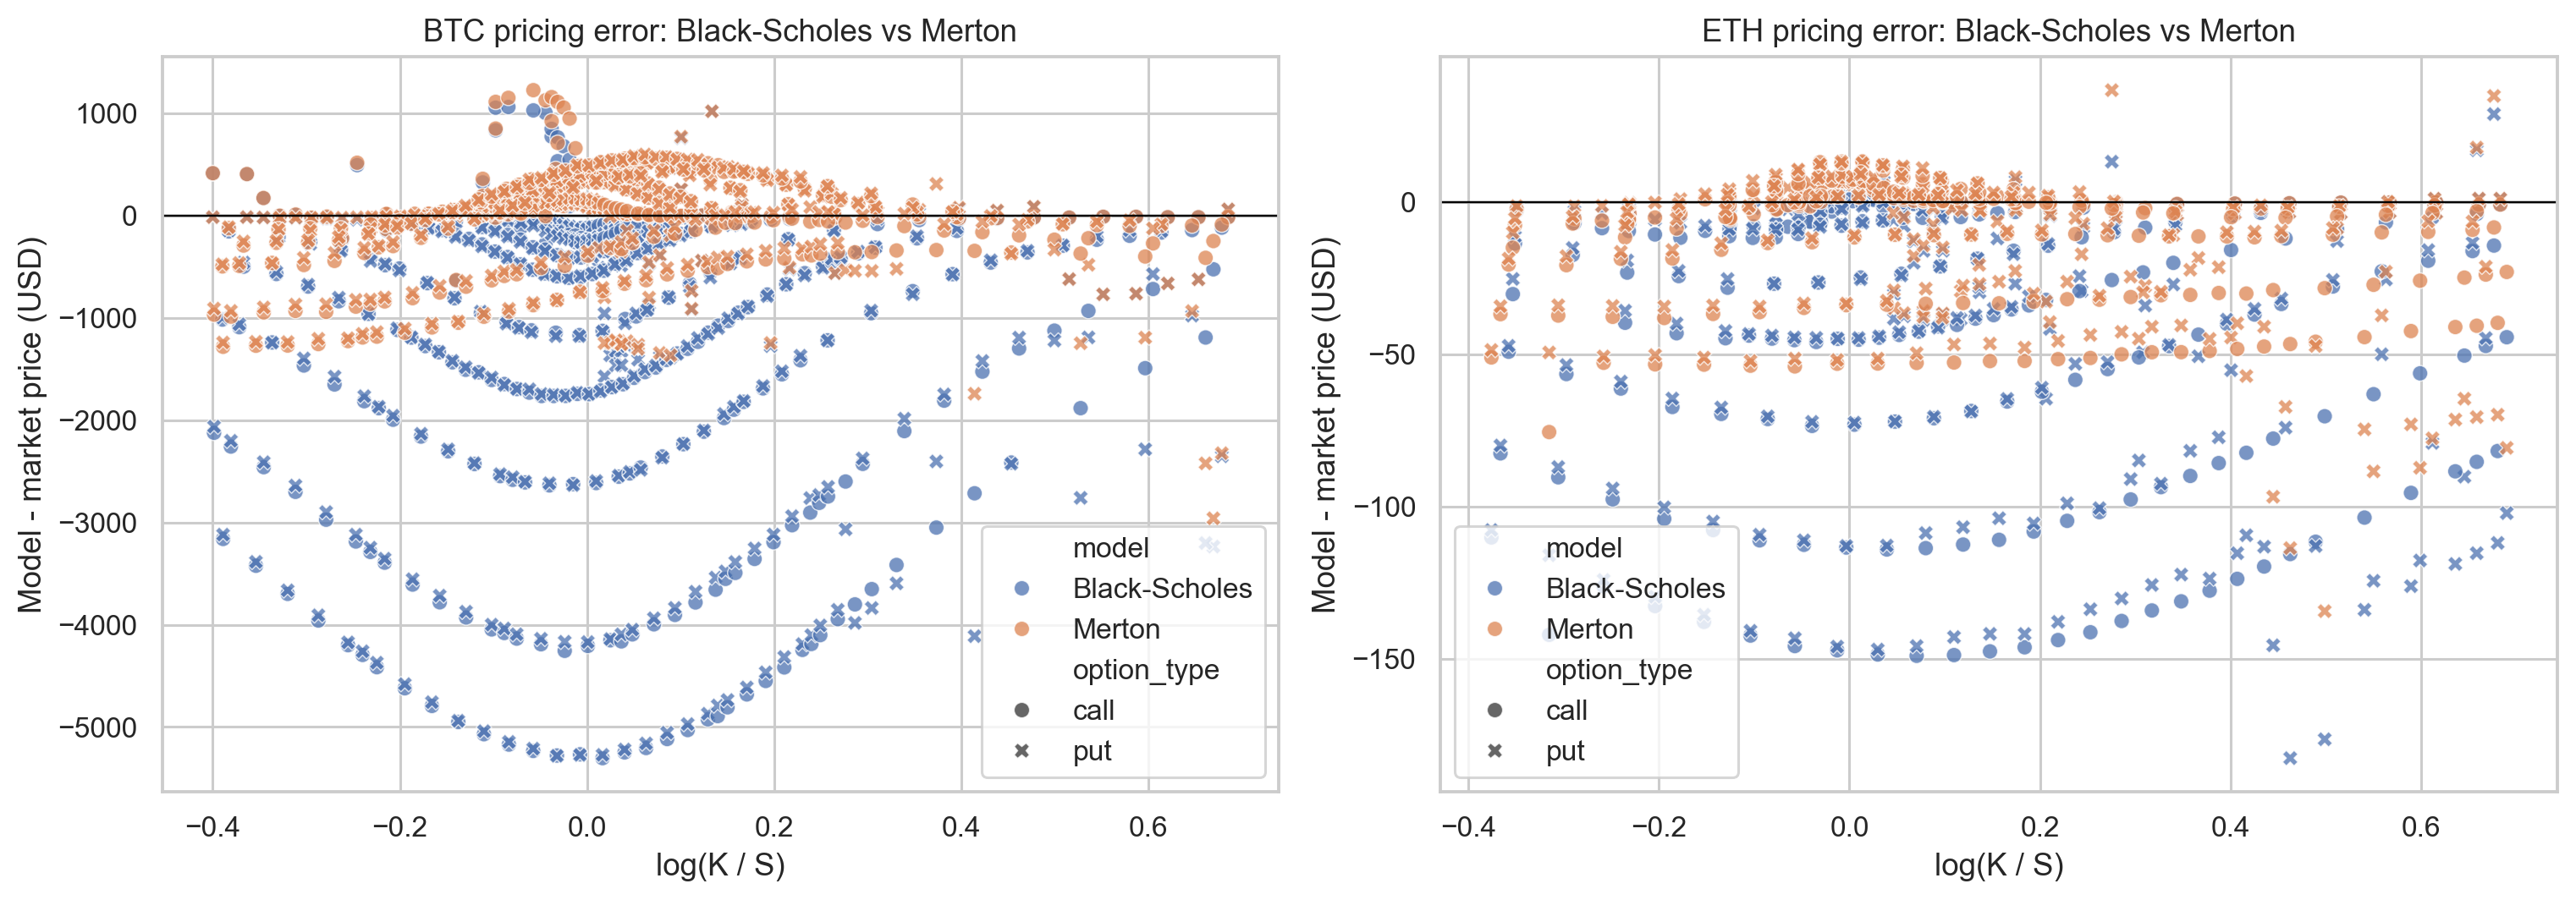
\includegraphics[width=0.98\linewidth]{figures/03_pricing_error_comparison.png}
\caption{Model pricing errors against Deribit option marks.}
\end{figure}

\begin{table}[H]
\centering
\caption{Candidate-level paired tests versus Black-Scholes absolute error}
\scriptsize
\begin{tabular}{llrrrrrr}
\toprule
Currency & Model & Pairs & Mean impr. & Median impr. & Share impr. & t-test p & Wilcoxon p\\
\midrule
BTC & Merton & 688 & \textbf{919.20} & 260.68 & 81.54\% & $2.18\times10^{-67}$ & $2.26\times10^{-85}$\\
BTC & SVCJ proxy & 688 & 918.29 & 235.39 & 82.27\% & $2.46\times10^{-65}$ & $1.52\times10^{-86}$\\
BTC & Dynamic jump & 688 & 881.75 & 312.51 & 85.76\% & $3.69\times10^{-75}$ & $1.51\times10^{-95}$\\
BTC & MR-ISVM surface & 688 & 781.36 & 292.08 & 80.09\% & $2.16\times10^{-62}$ & $1.54\times10^{-68}$\\
BTC & GARCH variance & 688 & 522.90 & 140.25 & 77.33\% & $7.84\times10^{-71}$ & $1.01\times10^{-75}$\\
ETH & MR-ISVM surface & 474 & \textbf{19.70} & 4.54 & 81.01\% & $1.27\times10^{-40}$ & $1.10\times10^{-42}$\\
ETH & Merton & 474 & 18.02 & 3.25 & 77.43\% & $4.03\times10^{-44}$ & $1.35\times10^{-38}$\\
ETH & Dynamic jump & 474 & 17.42 & 3.59 & 77.64\% & $5.48\times10^{-45}$ & $2.12\times10^{-39}$\\
ETH & GARCH variance & 474 & 17.08 & 3.57 & 85.65\% & $3.55\times10^{-48}$ & $2.97\times10^{-53}$\\
ETH & SVCJ proxy & 474 & 0.77 & 0.00 & 51.27\% & $2.02\times10^{-1}$ & $9.14\times10^{-1}$\\
\bottomrule
\end{tabular}
\end{table}

\begin{table}[H]
\centering
\caption{Full candidate pricing comparison on the cleaned option universe}
\scriptsize
\begin{tabular}{llrrrrrr}
\toprule
Currency & Model & Options & Bias & MAE & Median AE & RMSE & P90 AE\\
\midrule
BTC & \textbf{Merton} & 688 & -30.80 & \textbf{230.18} & 128.37 & 377.22 & 518.84\\
BTC & SVCJ proxy & 688 & 7.57 & 231.09 & 131.31 & 373.41 & 575.66\\
BTC & Dynamic jump & 688 & -156.60 & 267.63 & 112.46 & 464.34 & 787.05\\
BTC & MR-ISVM surface & 688 & -113.85 & 368.03 & 121.56 & 752.12 & 1061.42\\
BTC & GARCH variance & 688 & -616.22 & 626.48 & 268.89 & 982.65 & 1969.18\\
BTC & Black-Scholes & 688 & -1139.17 & 1149.38 & 498.17 & 1803.52 & 3612.63\\
ETH & \textbf{MR-ISVM surface} & 474 & -2.27 & \textbf{11.26} & 4.93 & 21.23 & 33.39\\
ETH & Merton & 474 & -9.58 & 12.94 & 5.28 & 21.47 & 40.31\\
ETH & Dynamic jump & 474 & -10.47 & 13.54 & 5.04 & 22.51 & 42.28\\
ETH & GARCH variance & 474 & -12.33 & 13.88 & 4.54 & 23.49 & 42.52\\
ETH & SVCJ proxy & 474 & 26.31 & 30.19 & 8.87 & 46.48 & 91.95\\
ETH & Black-Scholes & 474 & -30.76 & 30.96 & 10.89 & 49.51 & 95.11\\
\bottomrule
\end{tabular}
\end{table}

\begin{figure}[H]
\centering
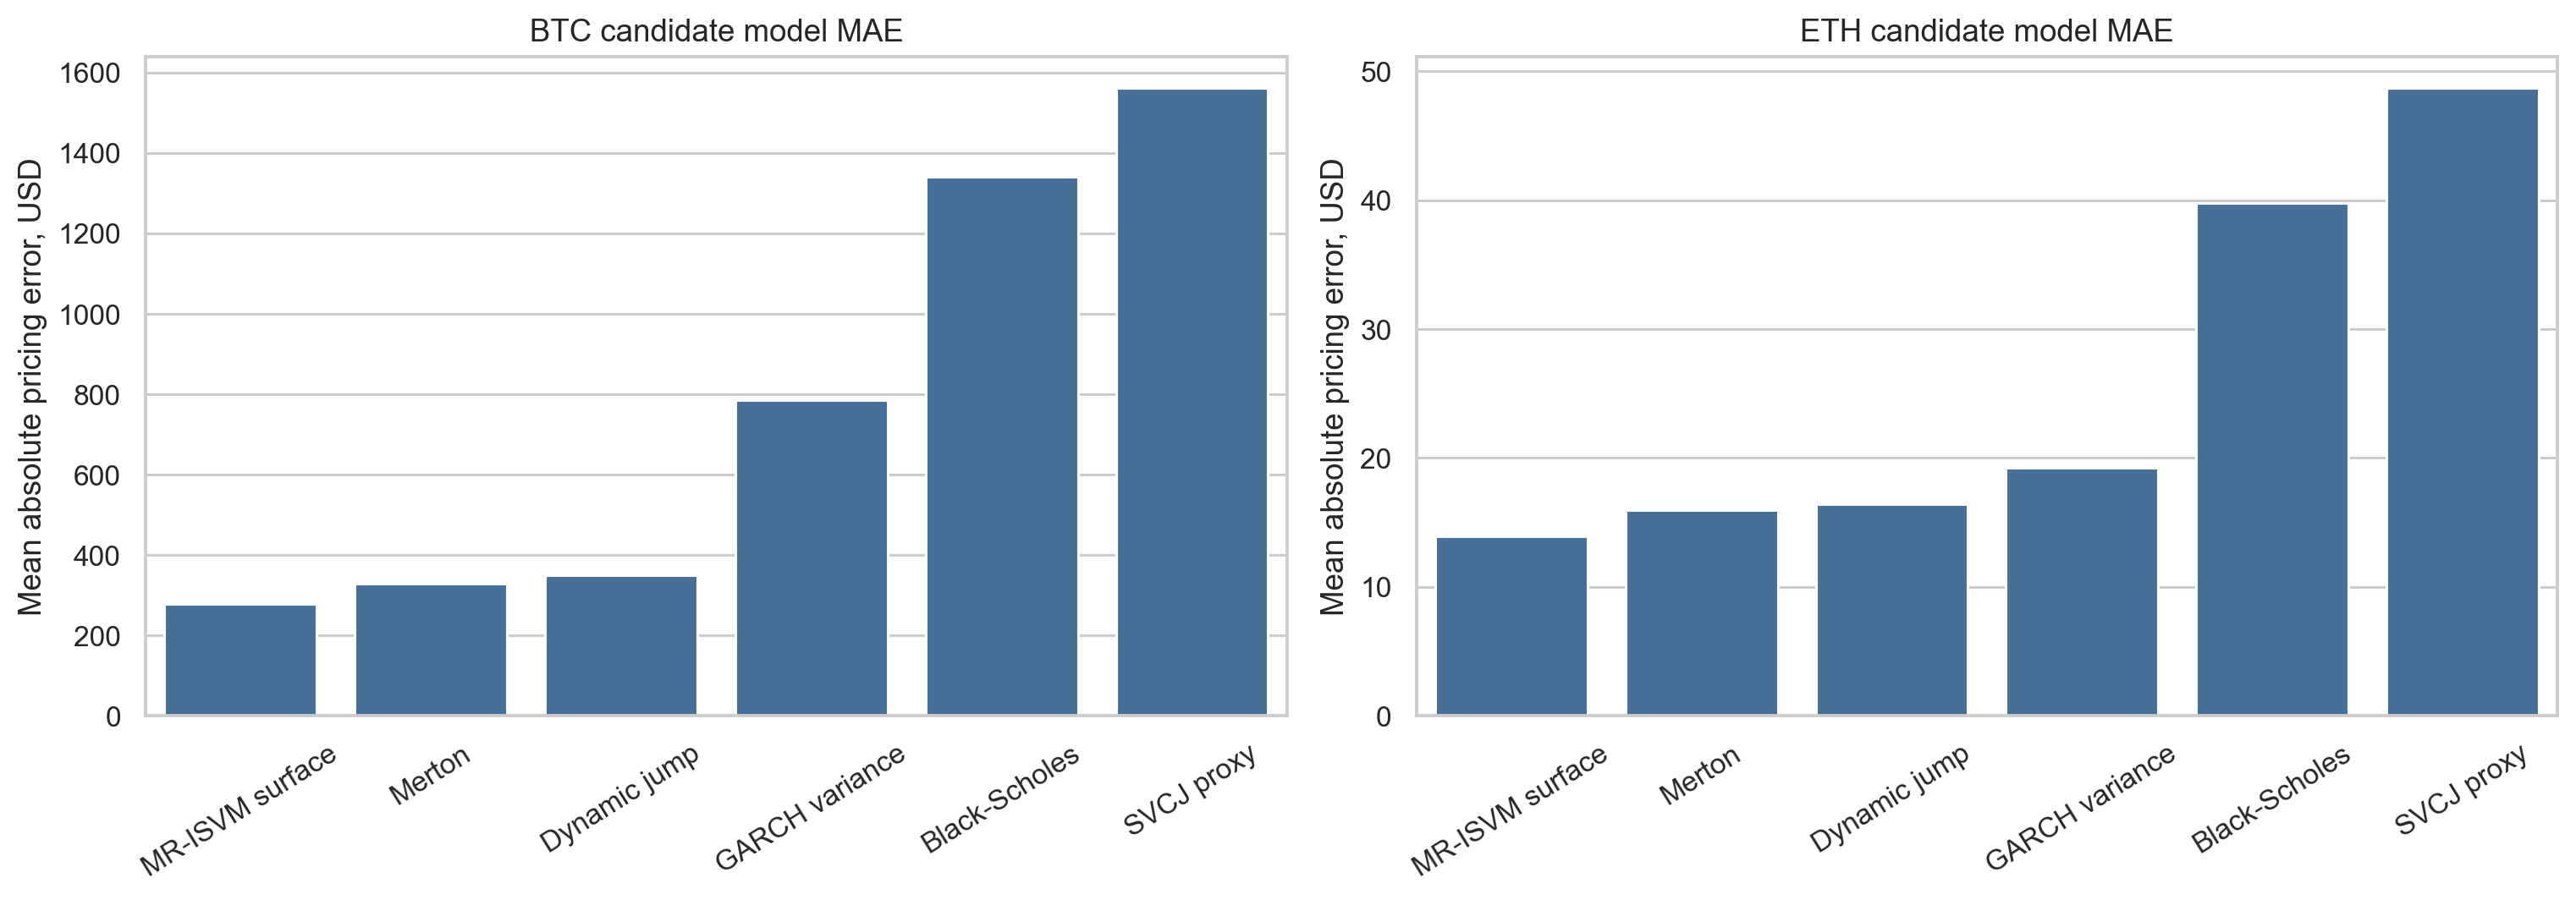
\includegraphics[width=0.98\linewidth]{figures/08_candidate_model_mae.png}
\caption{Equal-level candidate comparison using mean absolute pricing error.}
\end{figure}

\textbf{Inference.} The pricing improvement is not merely visual. Paired t-tests, Wilcoxon signed-rank tests, and sign tests show that most candidates reduce absolute pricing error relative to the Black-Scholes historical-volatility baseline. In this snapshot, Merton reduces BTC MAE from USD 1149.38 to USD 230.18; MR-ISVM reduces ETH MAE from USD 30.96 to USD 11.26.

The paired design is important. Each option is priced once by Black-Scholes and once by every candidate, so the test compares models instrument by instrument rather than comparing unrelated samples. This mirrors the course's emphasis on using a benchmark model first, then measuring model error against market prices.

\textbf{Comparative lens.} The broader candidate table changes the interpretation. Merton gives the best BTC MAE because the BTC cross section rewards a structural downside-jump premium. SVCJ is almost tied on BTC MAE and has the slightly lower BTC RMSE, meaning it helps on larger pricing misses but is marginally more expensive on average. MR-ISVM gives the best ETH MAE because the live ETH surface is better represented by a stress-regime implied-volatility map than by one jump distribution. GARCH improves materially over Black-Scholes by capturing volatility persistence, but it does not dominate the explicitly jump-aware or surface-aware candidates. The SVCJ proxy is not the ETH marking winner because it prices volatility-jump stress aggressively; that same conservatism becomes valuable in the crash-protection section.

\begin{table}[H]
\centering
\caption{Selected calibrated states for the modern candidates}
\scriptsize
\begin{tabular}{p{0.16\linewidth}p{0.38\linewidth}p{0.38\linewidth}}
\toprule
Model & BTC fitted state & ETH fitted state\\
\midrule
Merton & $\sigma=0.0300$, $\lambda=40.05$, $\mu_J=-0.0252$, $\delta_J=0.0635$ & $\sigma=0.3290$, $\lambda=40.05$, $\mu_J=-0.0349$, $\delta_J=0.0610$\\
SVCJ proxy & $v_0=0.0345$, $\theta=0.0009$, $\xi$ calibrated, multiplier $=0.250$ & $v_0=0.0989$, $\theta=0.1082$, $\xi$ calibrated, multiplier $=0.250$\\
MR-ISVM & active stress, two fitted fallback regimes, 12 coefficients, RMSE $=0.3699$ & active stress, two regimes, 12 coefficients, RMSE $=0.2783$\\
Dynamic jump & $\sigma=0.1586$, $\bar{\lambda}=31.76$, $\lambda_t=31.76$, $\beta=2.05$ & $\sigma=0.3602$, $\bar{\lambda}=33.01$, $\lambda_t=34.51$, $\beta=0.25$\\
GARCH variance & $\alpha+\beta=0.981$ & $\alpha+\beta=0.959$\\
\bottomrule
\end{tabular}
\end{table}

\section{Interest Rate Sensitivity}

We price 30-day at-the-money calls and puts under $r=1\%$ and $r=5\%$ to isolate interest-rate sensitivity. The table reports the price change from moving the annual risk-free rate from 1\% to 5\%, using the same calibrated state for every model.

\begin{table}[H]
\centering
\caption{All-candidate interest-rate sensitivity, $V(r=5\%)-V(r=1\%)$}
\small
\begin{tabular}{lrrrr}
\toprule
Model & BTC call & BTC put & ETH call & ETH put\\
\midrule
Black-Scholes & 125.32 & -126.96 & 3.35 & -3.59\\
Merton & 133.12 & -119.15 & 3.47 & -3.48\\
SVCJ proxy & 132.50 & -119.78 & 3.41 & -3.53\\
MR-ISVM surface & 123.55 & -129.59 & 3.36 & -3.61\\
Dynamic jump & 132.30 & -119.97 & 3.45 & -3.50\\
GARCH variance & 124.14 & -128.14 & 3.31 & -3.63\\
\bottomrule
\end{tabular}
\end{table}

\textbf{Inference.} Every model has the expected sign from put-call parity and discounting: higher rates increase calls and reduce puts. For a non-expert reader, the intuition is simple: a higher discount rate lowers the present value of the strike paid in the future, helping calls and hurting puts. Over a 30-day crypto horizon, however, the difference between models is driven much more by volatility, jumps, and surface shape than by the interest-rate input. This is a useful hierarchy of risks: for short-dated BTC/ETH options, the main modeling battle is not the risk-free rate, but the distribution of the underlying.

\textbf{Comparative lens.} The same hierarchy applies to the candidate models. Interest rates are a shared input, while the dominant disagreement across Black-Scholes, Merton, MR-ISVM, SVCJ, dynamic jump intensity, and GARCH comes from the assumed distribution of $S_T$. This is why we evaluate both average pricing error and standardized crash-protection values.

\section{Jump-Parameter Sensitivity}

We stress the calibrated Merton model by repricing 30-day, 5\% out-of-the-money puts under different jump-intensity and jump-volatility multipliers. This directly measures the value of crash protection.

\begin{figure}[H]
\centering
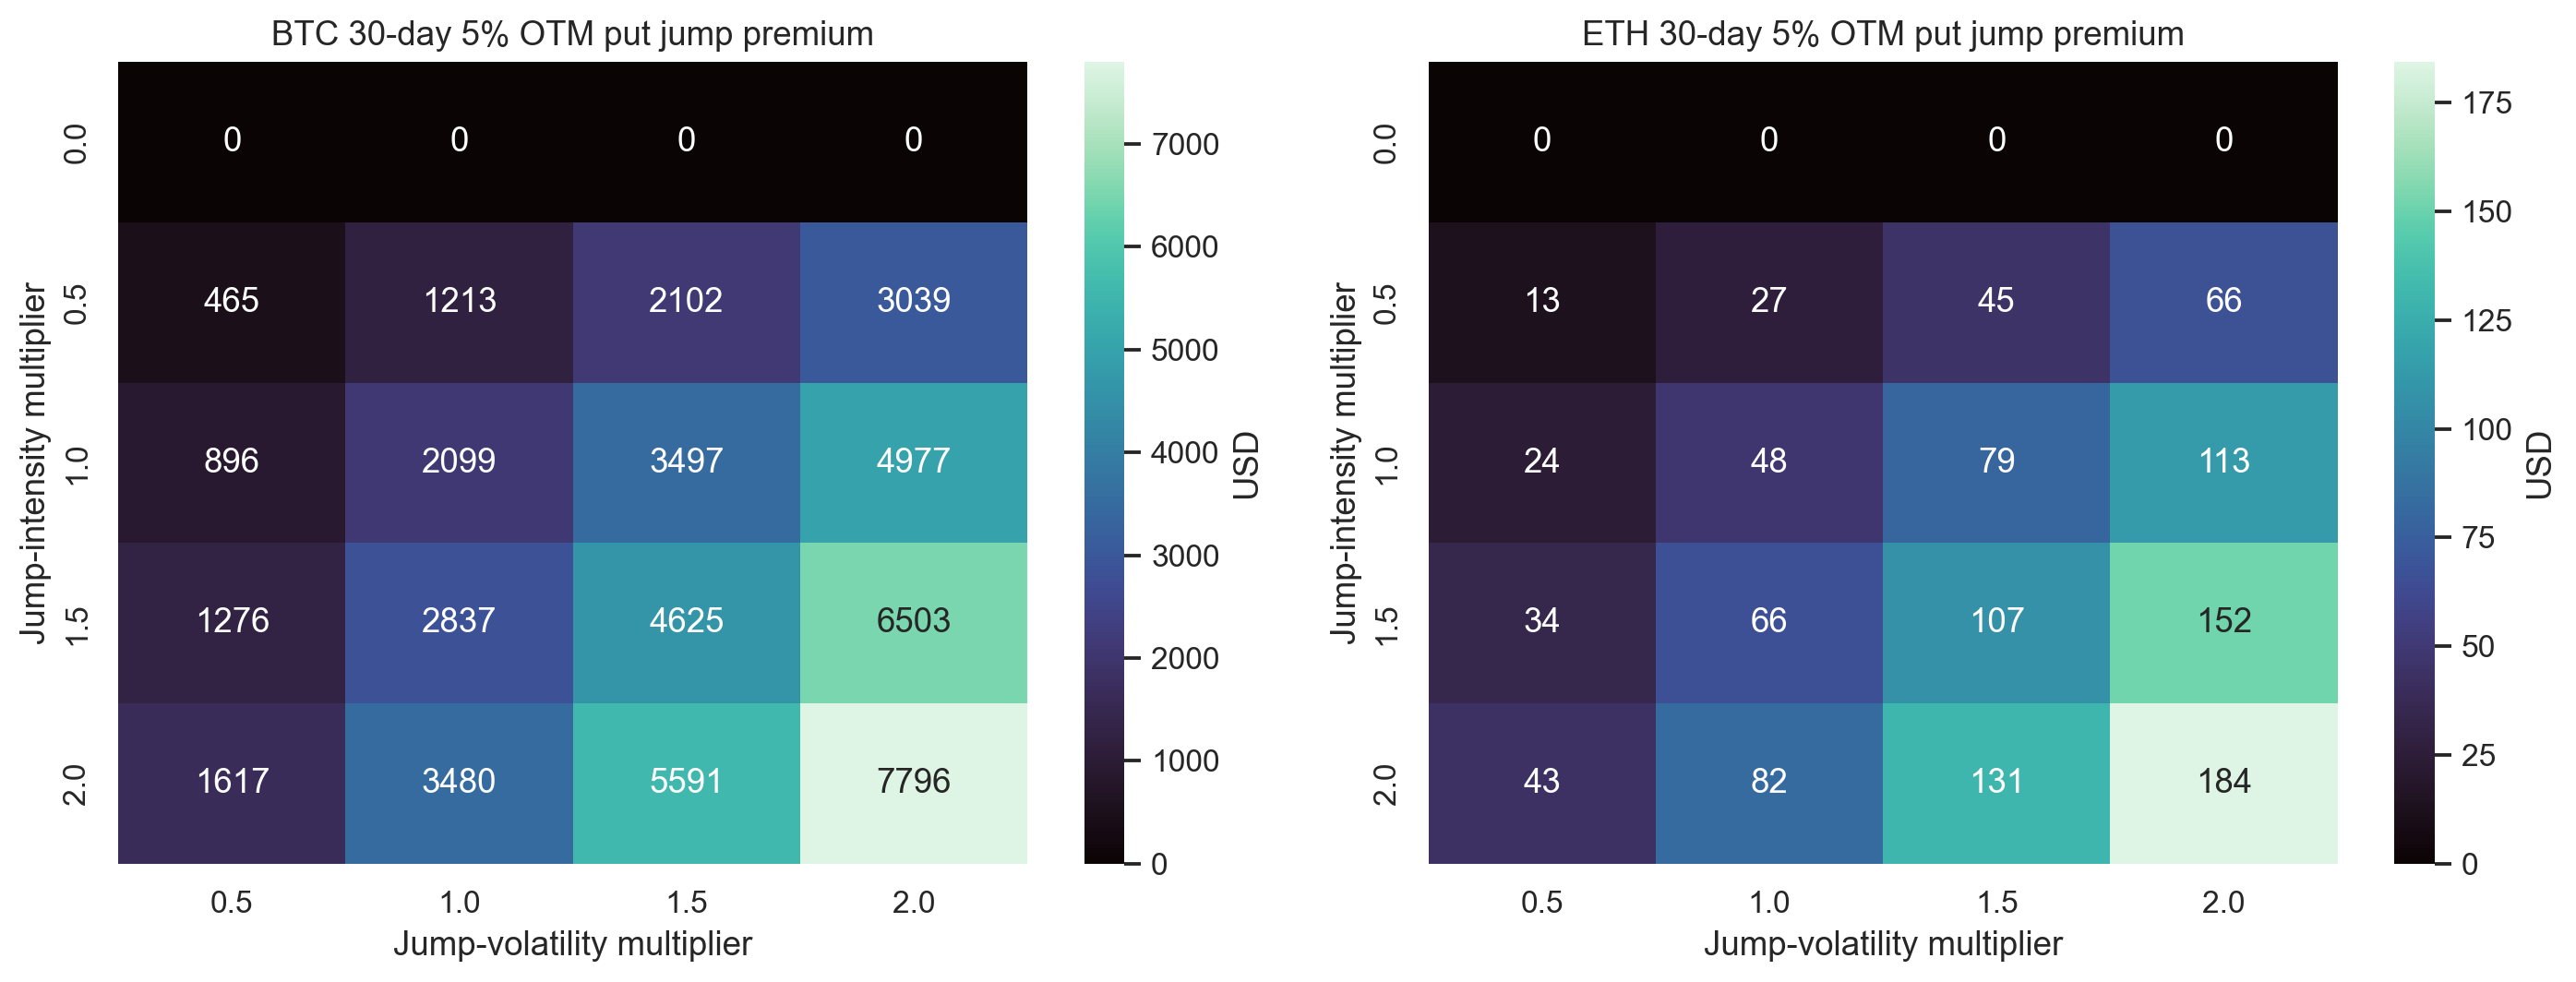
\includegraphics[width=0.98\linewidth]{figures/07_jump_parameter_sensitivity.png}
\caption{Sensitivity of 30-day 5\% OTM put jump premium to jump intensity and jump-size volatility.}
\end{figure}

\textbf{Inference.} The jump premium rises nonlinearly as either jump intensity or jump-size volatility increases. For BTC, doubling both calibrated jump intensity and jump volatility increases the 30-day 5\% OTM put premium by about USD 7796 relative to the low-diffusion baseline implied by the calibrated Merton state. For ETH, the comparable premium is about USD 184. This is a compact risk-management result: crash protection is primarily a jump-risk instrument, not just a high-volatility instrument.

The Risk Management chapter brings this sensitivity analysis into model-risk language. Greeks measure local sensitivities, but a jump parameter shock is a structural stress test. The heatmap therefore complements Delta and Vega: it asks how much the option value changes when the assumed tail process itself becomes more severe.

\begin{table}[H]
\centering
\caption{Standardized 30-day 5\% OTM put values across candidates}
\small
\begin{tabular}{llrr}
\toprule
Currency & Model & Put value & Premium over BS\\
\midrule
BTC & Black-Scholes & 900.47 & 0.00\\
BTC & Merton & 2098.74 & 1198.27\\
BTC & \textbf{SVCJ proxy} & \textbf{2145.55} & \textbf{1245.08}\\
BTC & MR-ISVM surface & 1963.21 & 1062.74\\
BTC & Dynamic jump & 1960.79 & 1060.32\\
BTC & GARCH variance & 1249.04 & 348.57\\
ETH & Black-Scholes & 58.77 & 0.00\\
ETH & Merton & 83.19 & 24.41\\
ETH & \textbf{SVCJ proxy} & \textbf{92.48} & \textbf{33.70}\\
ETH & MR-ISVM surface & 72.37 & 13.60\\
ETH & Dynamic jump & 81.98 & 23.21\\
ETH & GARCH variance & 75.45 & 16.68\\
\bottomrule
\end{tabular}
\end{table}

\begin{figure}[H]
\centering
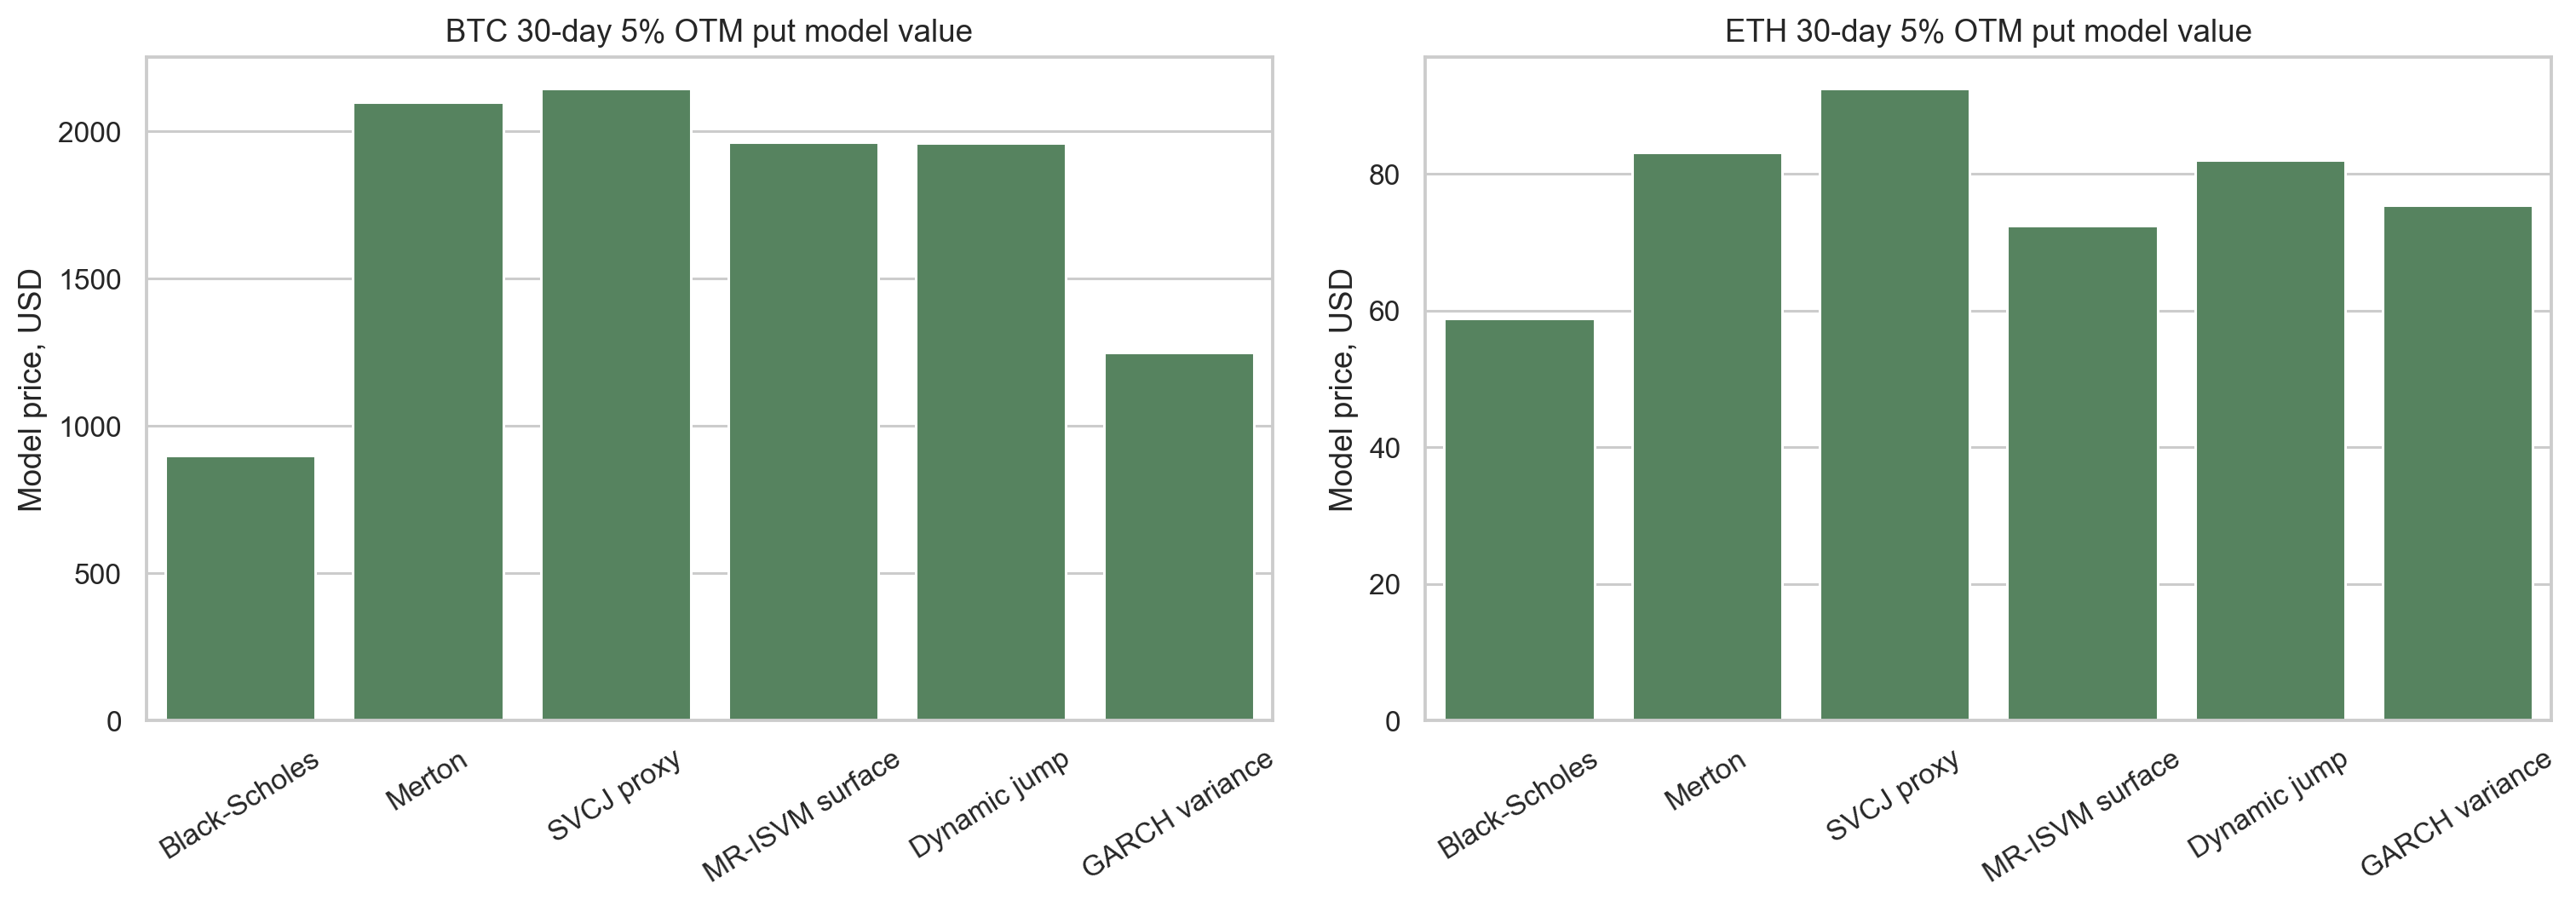
\includegraphics[width=0.98\linewidth]{figures/09_candidate_stress_puts.png}
\caption{Model-implied crash-protection values for standardized 30-day 5\% OTM puts.}
\end{figure}

\textbf{Comparative lens.} The ranking changes when the objective is crash protection rather than average pricing error. SVCJ produces the largest 30-day downside protection value because it prices the joint event ``spot falls and volatility jumps.'' Merton and dynamic jump intensity also attach large value to discontinuous downside moves. GARCH is more conservative because volatility clustering alone does not create jump losses. MR-ISVM sits between these cases: it reads the current market smile, but it does not explicitly simulate jump arrival.

\section{Greeks and Risk Management}

In the course framework, Greeks are sensitivities of option value to state variables and parameters. We compute Black-Scholes Greeks analytically and use finite differences for the candidate models so that the comparison is on the same footing. For the modern candidates, Vega is reported as a \emph{parallel volatility-input Vega}: the value change for a small bump to the model's effective volatility or implied-volatility input while keeping jump parameters fixed.

\begin{table}[H]
\centering
\caption{All-candidate Greeks for 30-day at-the-money puts at $r=1\%$}
\small
\begin{tabular}{llrrrr}
\toprule
Currency & Model & $\Delta$ & $\Gamma$ & Parallel vol Vega & Rho\\
\midrule
BTC & Black-Scholes & -0.4801 & 0.0000657 & 8789.99 & -3231.62\\
BTC & Merton & -0.4303 & 0.0000432 & 630.75 & -3018.16\\
BTC & SVCJ proxy & -0.4318 & 0.0000425 & 1685.93 & -3033.17\\
BTC & MR-ISVM surface & -0.4483 & 0.0085474 & 8783.18 & -3281.74\\
BTC & Dynamic jump & -0.4357 & 0.0000461 & 3560.77 & -3041.01\\
BTC & GARCH variance & -0.4780 & 0.0000557 & 8787.47 & -3253.27\\
ETH & Black-Scholes & -0.4723 & 0.0014892 & 241.64 & -90.85\\
ETH & Merton & -0.4433 & 0.0012249 & 148.54 & -87.79\\
ETH & SVCJ proxy & -0.4462 & 0.0011319 & 165.38 & -89.18\\
ETH & MR-ISVM surface & -0.4603 & 0.4778110 & 241.56 & -91.24\\
ETH & Dynamic jump & -0.4466 & 0.0012363 & 164.15 & -88.30\\
ETH & GARCH variance & -0.4683 & 0.0012685 & 241.46 & -91.68\\
\bottomrule
\end{tabular}
\end{table}

\begin{figure}[H]
\centering
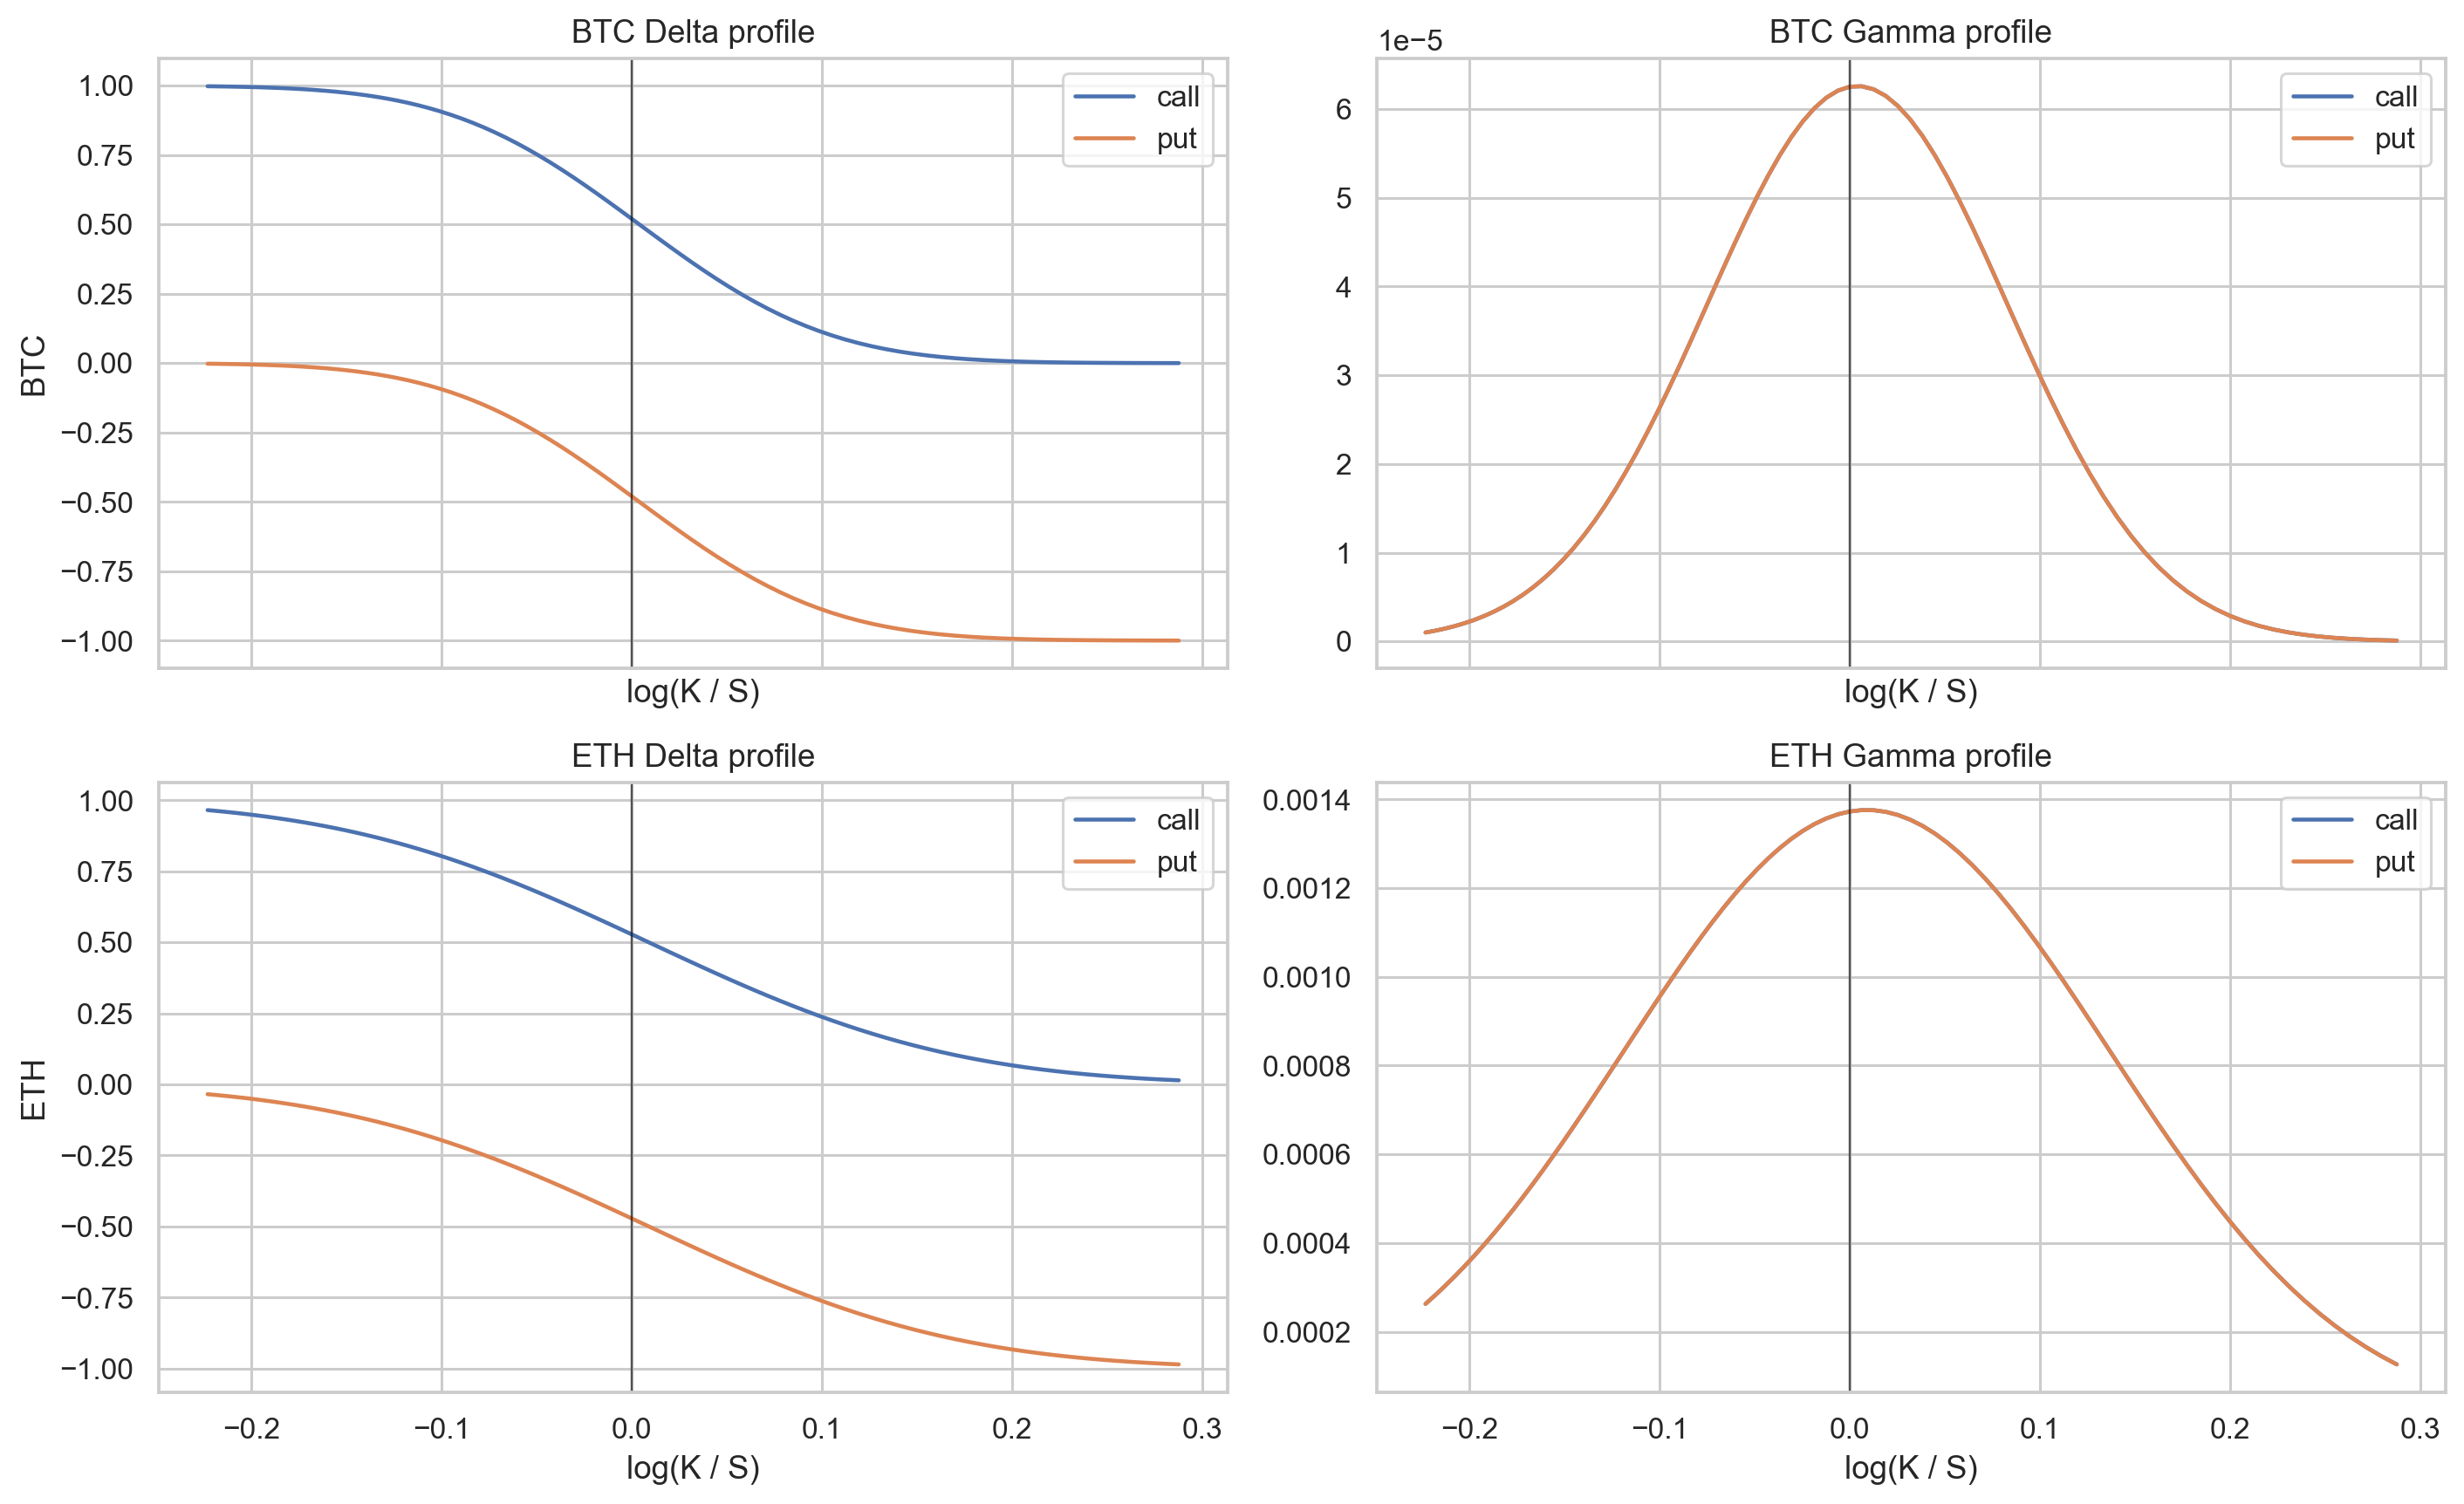
\includegraphics[width=0.98\linewidth]{figures/05_greek_profiles.png}
\caption{Black-Scholes Delta and Gamma profiles across log-moneyness.}
\end{figure}

\textbf{Inference.} Jump-aware put deltas are less negative than Black-Scholes deltas because some downside value is carried by jump states rather than only by local diffusion. In plain language, the model says: ``not every crash can be hedged by a tiny spot move.'' Gamma and Vega are also reallocated. Merton has low parallel-volatility Vega because much of the OTM put value is explained by jump intensity and jump size. MR-ISVM shows very high finite-difference Gamma because its surface delta includes the fitted smile changing as moneyness changes; this is a surface-risk Greek, not merely the textbook Black-Scholes curvature.

The course relation
\[
\Theta+rS\Delta+\frac{1}{2}\sigma^2S^2\Gamma=r\Pi
\]
is a useful interpretation device. Under pure diffusion, Delta and Gamma summarize the first two local spot risks. Under jumps, however, a finite move in $S$ can dominate the Taylor approximation. This is why the Greeks section must be read together with the jump-sensitivity and hedge-simulation sections.

\textbf{Comparative lens.} Greeks are local diagnostics, while candidate-model differences are partly global distributional assumptions. Black-Scholes and GARCH mainly modify the volatility channel; Merton and dynamic jump intensity modify the jump-arrival channel; SVCJ modifies both variance and jump channels; MR-ISVM embeds the market's current state into the implied-volatility surface. The practical implication is that a desk should not interpret Delta or Vega without also checking which model generated the distribution around those Greeks.

\section{Jump-Hedging Simulation}

Continuous delta hedging is an idealization. The Risk Management chapter notes that periodic hedging introduces replication error. We simulate 30-day, 5\% OTM put hedging under the same Merton jump paths for every candidate model. Each model supplies its own finite-difference Delta, and the hedge is rebalanced daily. This makes the comparison practical: it asks which model leaves the smaller residual P\&L when the underlying path contains jumps.

\begin{figure}[H]
\centering
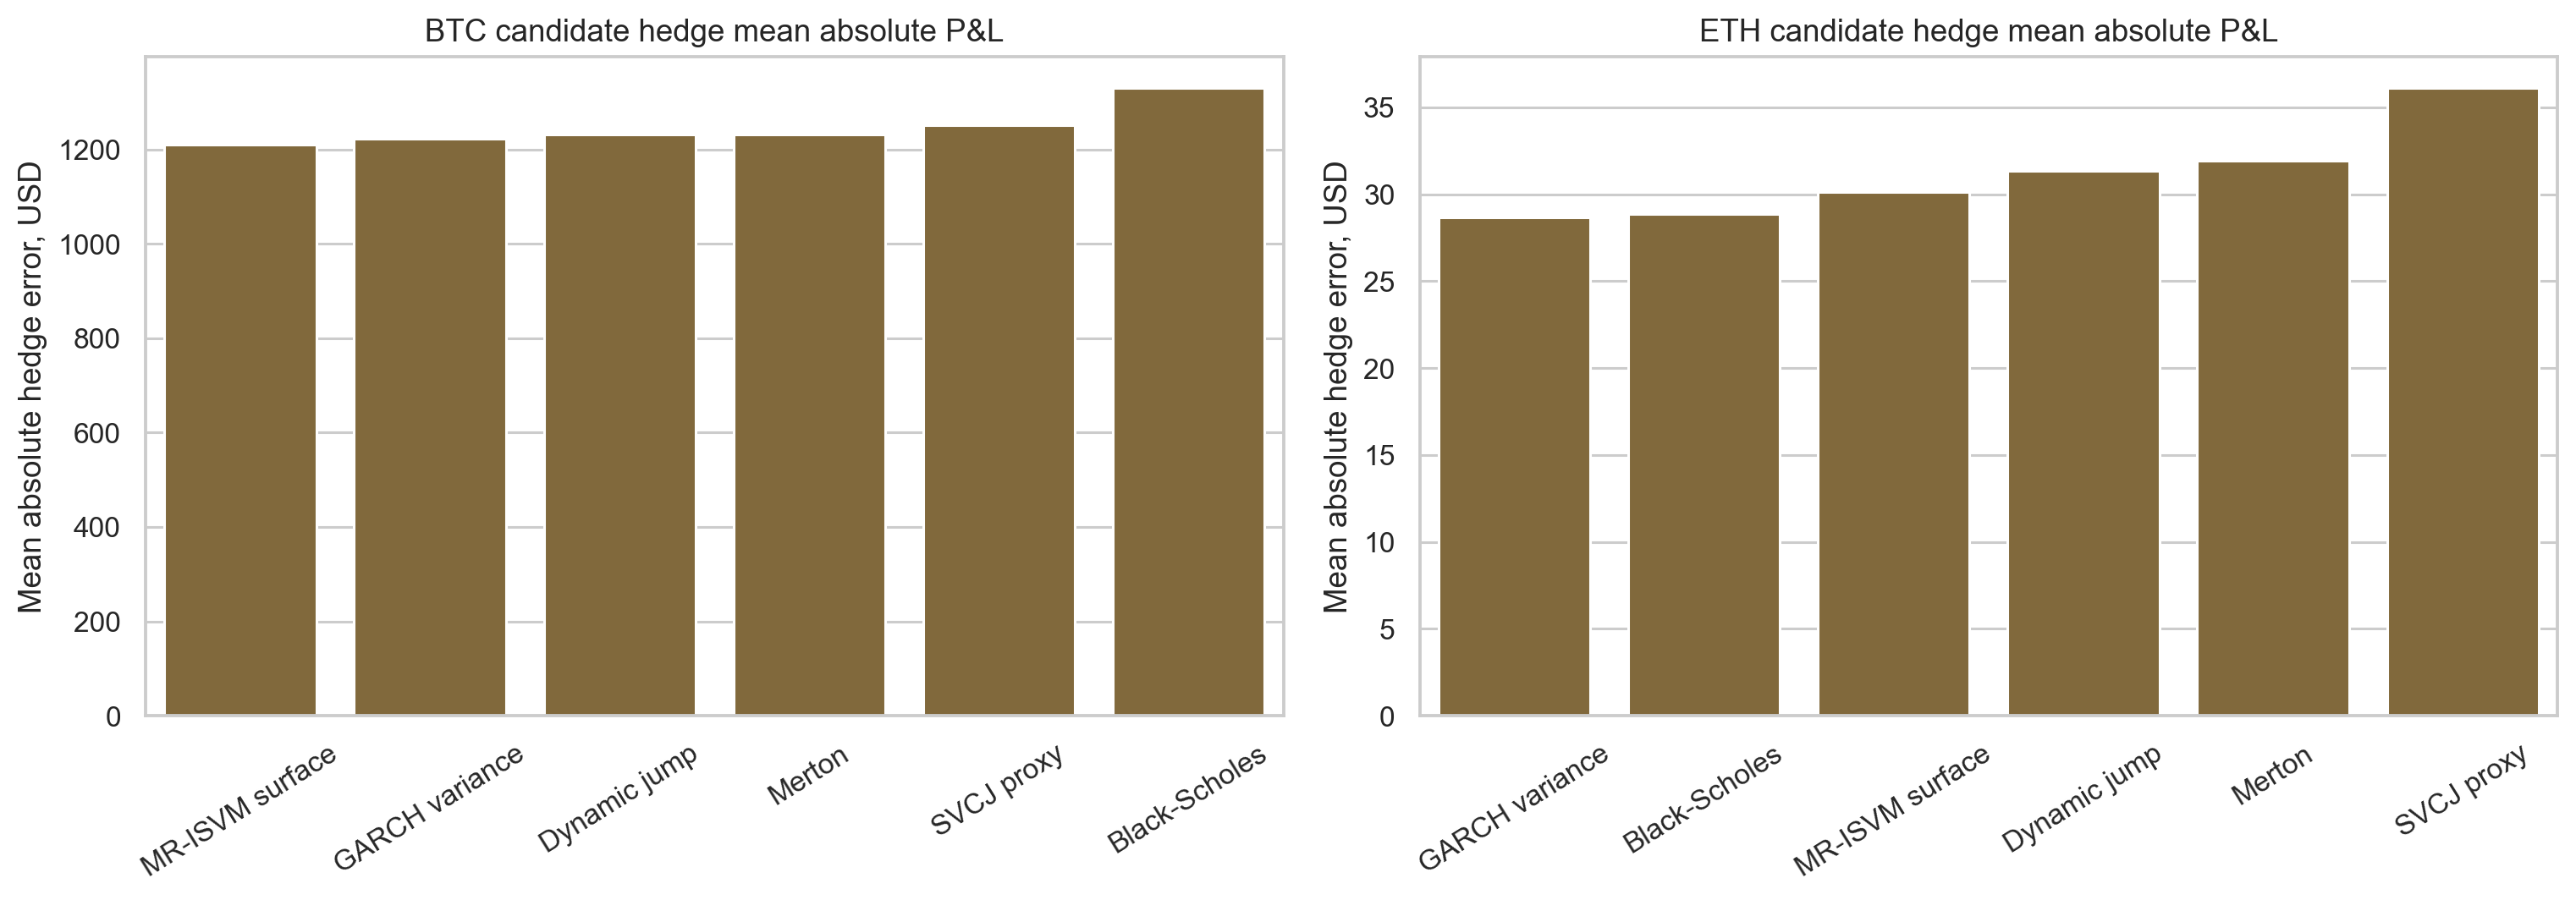
\includegraphics[width=0.92\linewidth]{figures/10_candidate_hedge_errors.png}
\caption{Mean absolute hedge error for all candidates under common Merton jump paths.}
\end{figure}

\begin{table}[H]
\centering
\caption{Candidate-level discrete hedge-error summary}
\small
\begin{tabular}{llrrrr}
\toprule
Currency & Model & Mean P\&L & Median P\&L & Mean $|$P\&L$|$ & 5\% P\&L\\
\midrule
BTC & \textbf{MR-ISVM surface} & -71.09 & 430.62 & \textbf{1209.79} & -3642.82\\
BTC & GARCH variance & -721.22 & -99.04 & 1221.90 & -4115.41\\
BTC & Dynamic jump & -76.15 & 532.40 & 1232.12 & -3433.50\\
BTC & Merton & 45.42 & 597.32 & 1232.37 & -3265.26\\
BTC & SVCJ proxy & 92.57 & 634.94 & 1251.67 & -3204.44\\
BTC & Black-Scholes & -1053.16 & -439.59 & 1330.13 & -4812.70\\
ETH & \textbf{GARCH variance} & -0.67 & 12.53 & \textbf{28.65} & -66.09\\
ETH & Black-Scholes & -17.09 & 0.77 & 28.84 & -95.27\\
ETH & MR-ISVM surface & -2.42 & 14.01 & 30.11 & -70.25\\
ETH & Dynamic jump & 6.09 & 17.00 & 31.33 & -60.94\\
ETH & Merton & 7.25 & 17.87 & 31.92 & -60.59\\
ETH & SVCJ proxy & 15.94 & 25.66 & 36.12 & -51.01\\
\bottomrule
\end{tabular}
\end{table}

\textbf{Inference.} Hedging gives a different ranking from pricing. \textbf{MR-ISVM has the lowest BTC mean absolute hedge error}, while \textbf{GARCH has the lowest ETH mean absolute hedge error}. SVCJ has the least negative 5\% tail P\&L for both assets, but its larger protection premium can raise average hedge error. This is a desk-level lesson: the best marking model, best stress model, and best hedge model need not be the same.

This result connects directly to the replication logic in the binomial and Black-Scholes chapters. Replication is exact only under the assumed dynamics and rebalancing frequency. Once the true path contains discontinuities, a self-financing delta hedge accumulates residual error. The practical question is therefore not whether hedging eliminates risk, but which model leaves the smaller residual under realistic crypto paths.

\textbf{Comparative lens.} All candidates are tested on the same simulated paths, but their economic roles differ. MR-ISVM adapts local deltas to the live surface; Merton and dynamic jump intensity make jump exposure explicit; SVCJ over-insures crash states and improves left-tail hedge P\&L; GARCH reacts through persistent conditional variance. Together, the comparison separates three desk questions: which model marks best, which model stresses tail protection most, and which model gives the most stable hedge.

\section{Discussion}

Black-Scholes is internally coherent under frictionless trading, continuous hedging, constant volatility, and lognormal diffusion. Crypto markets violate these assumptions in several ways:
\begin{itemize}
\item returns are heavy-tailed and negatively skewed;
\item volatility is regime-dependent;
\item investors pay for downside crash protection;
\item delta hedging is discrete and liquidity can vanish during stress;
\item leverage and liquidation effects can amplify short-horizon moves.
\end{itemize}

The Merton model is therefore not an ornamental extension. It is a mathematically controlled way to carry the course's risk-neutral framework into the empirical reality of BTC/ETH options. But the equal-level candidate comparison also shows why Merton should not be the final word. Merton currently gives the cleanest BTC cross-sectional MAE; MR-ISVM gives the cleanest ETH cross-sectional MAE; SVCJ is more explicit about volatility jumps and dominates in standardized crash-premium analysis; dynamic intensity targets jump clustering; and GARCH isolates volatility persistence as a competing explanation. The hedge simulation adds one more layer: a model that is best for marking may not be best for residual hedge P\&L.

The sequence of chapters brings the analysis to a layered conclusion: risk-neutral pricing tells us how to value claims once dynamics are specified; binomial trees show how replication works discretely; Black-Scholes gives the diffusion benchmark; implied volatility reveals the benchmark's market misfit; and risk management exposes the hedging cost of that misfit. The model-comparison layer is our response to that chain of evidence.

\section{Conclusion}

This project implements a complete option pricing workflow: Black-Scholes prices and Greeks, CRR European and American trees, implied-volatility smiles, market calibration, candidate model comparison, and dynamic hedge simulation.

The innovation is no longer only the Merton jump-diffusion layer. It is the equal-level comparison of six pricing views: diffusion, constant jump intensity, stochastic volatility jumps, regime implied volatility, dynamic jump intensity, and GARCH conditional variance.

The central finding is that crypto option markets price jump risk and volatility-regime risk explicitly. Black-Scholes should be treated as a control model and teaching benchmark. A professional crypto options desk would not select one model for every purpose: it would use the best surface or structural model for marking, then retain jump and SVCJ-style engines for stress testing, Greeks, and risk management.

\newpage
\begin{thebibliography}{99}

\bibitem{bates1996}
Bates, D. S. (1996).
Jumps and stochastic volatility: Exchange rate processes implicit in Deutsche Mark options.
\emph{The Review of Financial Studies}, 9(1), 69--107.

\bibitem{blackscholes1973}
Black, F., and Scholes, M. (1973).
The pricing of options and corporate liabilities.
\emph{Journal of Political Economy}, 81(3), 637--654.

\bibitem{chenyang2024}
Chen, K. S., and Yang, J. J. (2024).
Price dynamics and volatility jumps in bitcoin options.
\emph{Financial Innovation}, 10, Article 132.

\bibitem{coxrossrubinstein1979}
Cox, J. C., Ross, S. A., and Rubinstein, M. (1979).
Option pricing: A simplified approach.
\emph{Journal of Financial Economics}, 7(3), 229--263.

\bibitem{duffie2000}
Duffie, D., Pan, J., and Singleton, K. (2000).
Transform analysis and asset pricing for affine jump-diffusions.
\emph{Econometrica}, 68(6), 1343--1376.

\bibitem{hou2020crypto}
Hou, A. J., Wang, W. N., Chen, C. Y.-H., and H\"ardle, W. K. (2020).
Pricing cryptocurrency options.
\emph{Journal of Financial Econometrics}, 18(2), 250--279.

\bibitem{jiang2026lecture}
Jiang, W. (2026).
IEDA4331 Financial Engineering lecture notes: risk-neutral pricing, binomial trees, Black-Scholes-Merton, and risk management.
Hong Kong University of Science and Technology.

\bibitem{merton1973}
Merton, R. C. (1973).
Theory of rational option pricing.
\emph{The Bell Journal of Economics and Management Science}, 4(1), 141--183.

\bibitem{merton1976}
Merton, R. C. (1976).
Option pricing when underlying stock returns are discontinuous.
\emph{Journal of Financial Economics}, 3(1--2), 125--144.

\bibitem{saef2022mrisvm}
Saef, D., Wang, Y., and Aste, T. (2022).
Regime-based implied stochastic volatility model for crypto option pricing.
arXiv:2208.12614.

\bibitem{venter2020garch}
Venter, P. J., and Mar\'e, E. (2021).
Univariate and multivariate GARCH models applied to Bitcoin futures option pricing.
\emph{Journal of Risk and Financial Management}, 14(6), Article 261.

\bibitem{zulfiqar2021iv}
Zulfiqar, N., and Gulzar, S. (2021).
Implied volatility estimation of Bitcoin options and the stylized facts of option pricing.
\emph{Financial Innovation}, 7, Article 67.

\end{thebibliography}

\clearpage
\appendix
\section{Implementation Notes}

The implementation is modular:
\begin{itemize}
\item \texttt{src/data\_deribit.py}: public Deribit data access and caching.
\item \texttt{src/preprocessing.py}: quote cleaning, USD conversion, returns, and jump detection.
\item \texttt{src/black\_scholes.py}, \texttt{src/binomial.py}, and \texttt{src/merton\_jump.py}: baseline and jump pricing engines.
\item \texttt{src/candidate\_models.py}: comparable modern candidates.
\item \texttt{src/calibration.py} and \texttt{src/risk.py}: calibration and hedge simulation.
\item \texttt{scripts/generate\_report\_assets.py}: reproducible report tables and figures.
\end{itemize}

\clearpage
\section{Core Programming Code Listings}

This appendix records the key programming modules that implement the report's pricing, calibration, candidate-model, and risk-management analysis. The listings are selected source excerpts rather than every helper function in the repository; each one is labelled so the implementation can be traced directly to the mathematical sections of the report.

\lstinputlisting[
  style=pythoncode,
  firstline=65,
  lastline=105,
  firstnumber=65,
  caption={Data client for Deribit public market-data requests.},
  label={lst:data-client}
]{../src/data_deribit.py}

\lstinputlisting[
  style=pythoncode,
  firstline=29,
  lastline=106,
  firstnumber=29,
  caption={Option-chain normalization: metadata merge, USD conversion, maturity, moneyness, and IV features.},
  label={lst:preprocessing-option-chain}
]{../src/preprocessing.py}

\lstinputlisting[
  style=pythoncode,
  firstline=135,
  lastline=158,
  firstnumber=135,
  caption={Historical return construction and robust jump detection.},
  label={lst:preprocessing-jumps}
]{../src/preprocessing.py}

\lstinputlisting[
  style=pythoncode,
  firstline=53,
  lastline=160,
  firstnumber=53,
  caption={Black-Scholes pricing and analytic Greeks.},
  label={lst:black-scholes}
]{../src/black_scholes.py}

\lstinputlisting[
  style=pythoncode,
  firstline=163,
  lastline=212,
  firstnumber=163,
  caption={Black-Scholes implied-volatility inversion by robust bisection.},
  label={lst:implied-vol}
]{../src/black_scholes.py}

\lstinputlisting[
  style=pythoncode,
  firstline=17,
  lastline=87,
  firstnumber=17,
  caption={CRR binomial tree engine with European/American exercise support and convergence diagnostics.},
  label={lst:crr-tree}
]{../src/binomial.py}

\lstinputlisting[
  style=pythoncode,
  firstline=14,
  lastline=96,
  firstnumber=14,
  caption={Merton jump-diffusion parameters and Poisson-mixture pricing engine.},
  label={lst:merton-price}
]{../src/merton_jump.py}

\lstinputlisting[
  style=pythoncode,
  firstline=99,
  lastline=174,
  firstnumber=99,
  caption={Merton finite-difference Greeks and risk-neutral path simulation.},
  label={lst:merton-greeks-paths}
]{../src/merton_jump.py}

\lstinputlisting[
  style=pythoncode,
  firstline=41,
  lastline=76,
  firstnumber=41,
  caption={Historical initialization of Merton parameters from index returns.},
  label={lst:merton-historical-init}
]{../src/calibration.py}

\lstinputlisting[
  style=pythoncode,
  firstline=101,
  lastline=184,
  firstnumber=101,
  caption={Market calibration of Merton parameters to Deribit option prices.},
  label={lst:merton-calibration}
]{../src/calibration.py}

\lstinputlisting[
  style=pythoncode,
  firstline=83,
  lastline=335,
  firstnumber=83,
  caption={MR-ISVM 12-factor implied-volatility surface fit and Black-Scholes repricing.},
  label={lst:mrisvm-surface}
]{../src/candidate_models.py}

\lstinputlisting[
  style=pythoncode,
  firstline=344,
  lastline=690,
  firstnumber=344,
  caption={Regime detection and multi-regime MR-ISVM surface wrapper.},
  label={lst:mrisvm-regime}
]{../src/candidate_models.py}

\lstinputlisting[
  style=pythoncode,
  firstline=790,
  lastline=995,
  firstnumber=790,
  caption={SVCJ moment proxy, identifiable calibration, and Merton-layered pricing.},
  label={lst:svcj-proxy}
]{../src/candidate_models.py}

\lstinputlisting[
  style=pythoncode,
  firstline=998,
  lastline=1163,
  firstnumber=998,
  caption={Dynamic jump-intensity pricing and equal-level candidate error summaries.},
  label={lst:dynamic-and-candidate-summary}
]{../src/candidate_models.py}

\lstinputlisting[
  style=pythoncode,
  firstline=55,
  lastline=137,
  firstnumber=55,
  caption={Discrete delta-hedging simulation for short options.},
  label={lst:delta-hedge}
]{../src/risk.py}

\lstinputlisting[
  style=pythoncode,
  firstline=140,
  lastline=181,
  firstnumber=140,
  caption={Jump-path hedge experiment comparing Black-Scholes and Merton hedges.},
  label={lst:jump-hedge-experiment}
]{../src/risk.py}

\lstinputlisting[
  style=pythoncode,
  firstline=380,
  lastline=572,
  firstnumber=380,
  caption={All-candidate diagnostic pricing, finite-difference Greeks, and hedge-path logic used in the report comparison.},
  label={lst:candidate-diagnostics}
]{../scripts/generate_report_assets.py}

\section{AI Assistance Statement}

AI assistance was used to structure the project, implement Python modules, develop explanatory text, generate plots and tables, and format this report. The quantitative formulas, course alignment, market data, statistical tests, and validation checks are explicit in the codebase and report. The implementation was verified with unit tests and live Deribit data smoke tests.

\end{document}
